\documentclass{article}
\usepackage[layout=letterpaper,margin=1in]{geometry}

\usepackage{bold-extra} % for bf sc

\usepackage{fancyhdr}
\usepackage{xspace}
\usepackage{color}
\usepackage{graphicx}
\usepackage{subcaption}
\usepackage{comment}
\usepackage{soul} % provides \hl{}
\usepackage{listings}

\usepackage[section]{placeins} % Don't let figs escape their section

\usepackage[colorlinks=true]{hyperref}

\usepackage[all=normal,lists]{savetrees}

\usepackage[endianness=big]{bytefield}
\bytefieldsetup{boxformatting={\centering\footnotesize}}

\usepackage{multirow}
\usepackage{tabularx}
\usepackage{nth}
\usepackage{moresize}
\usepackage{framed}

\usepackage{
  tikz,
  tikz-timing,
}
\usetikzlibrary{positioning}

\usepackage[nofancy]{svninfo}

\newcommand{\colorbitbox}[3]{%
\rlap{\bitbox{#2}{\color{#1}\rule{\width}{\height}}}%
\bitbox{#2}{#3}}
\definecolor{lightblue}{RGB}{0,204,255}
\definecolor{lightcyan}{rgb}{0.84,1,1}
\definecolor{lightgreen}{rgb}{0.64,1,0.71}
\definecolor{lightergreen}{rgb}{0.84,1,0.87}
\definecolor{lightred}{rgb}{1,0.7,0.71}

\definecolor{OliveGreen}{cmyk}{0.64,0,0.95,0.40}

\usepackage{enumitem}
\setlistdepth{8}
%\setlist[itemize,1]{label=$\bullet$}
\setlist[itemize,1]{label=}
\setlist[itemize,2]{label=--}
\setlist[itemize,3]{label=$\circ$}
\setlist[itemize,4]{label=$\rightarrow$}
\setlist[itemize,5]{label=$\diamondsuit$}
\setlist[itemize,6]{label=$\cdot$}
\setlist[itemize,7]{label=$\star$}
\setlist[itemize,8]{label=$\ast$}
\renewlist{itemize}{itemize}{8}

\newcommand{\bus}{ULPB\xspace}

%%%%%%%%%%%%%%%%%%%%%%%%%%%%%%%%%%%%%%%%%%%%%%%%%%%%%%%%%%%%%%%%%%%%%%%%%%%%%%%%
\begin{document}

\svnInfo $Id$ 

\fancyfoot[L]{Revision 0.5 -- \today}
\fancyfoot[R]{\footnotesize{\em (svn: \svnInfoFile::r\svnInfoRevision)}}
\pagestyle{fancyplain}

% XXX Temp, contents look silly with only one entry on a blank page
\title{\vspace{-1em} Ultra Low Power Bus}
\author{(Needs better name...)}
\date{}
\maketitle

\tableofcontents
\clearpage

\svnInfo $Id$

\section{Requirements \& Design Considerations}
\label{sec:requirements}
\label{sec:design}
This section attempts to explain the design tradeoffs made in the \bus design.

\paragraph{Define bus PHY, MAC and application logic interface}
We take a vertical integration approach, controlling more of the complete
stack in an effort to obtain every available ounce of energy efficiency within
our further design constraints.

\paragraph{Must be fully-synthesizable}
In an effort to make \bus ubiquitous, it is important that other designers can
easily add \bus to their systems/chips. In practice, this means a
fully-synthesizable design such that simple, pure Verilog can be given to any
individual wishing to implement \bus. The provides added advantages in
pre-silicon testing and validation.

\paragraph{Optimize for synthesis simplicity over speed}
The synthesizability is paramount. As example, standard cell libraries contain
both positive and negative edge triggered flip-flops, but a dual-edge
flip-flop is not available in many processes. It is important then that no
element of \bus design require an implementation that double-clocks flops.

\paragraph{Must be low-power, low-leakage}
The \bus was designed for the Michigan Micro Mote~(M3) project. The system is
designed to run off a 0.5~$\mu$Ah battery. To serve as a feasible
communication bus, the energy consumption must be on the order of $pW$.

This extreme power constraint eliminates traditional analog open-collector
style designs as options. Sufficiently low-leakage circuits would have
untenable drive strength requirements and/or rise time constraints. The
previously stated portability requirements eliminate custom crafted analog
elements as an option, restricting \bus design to a purely digital approach.
%XXX: Ballpark expected transaction sizes, frequency, etc -- actual energy budget.

\paragraph{Support Multi-master operation / bus arbitration / avoid race
conditions}
As every layer is capable of entering an extreme low-power state, any layer
must be capable of waking the system. The waking layer must also be capable of
communicating (i) who woke the system and (ii) why. While such a system could
query (ii) given (i), determining who woke the system requires a complex
dedicated controller, or for the waking layer to simply announce it. A
multi-master bus greatly simplifies the software design and allows for things
such as DMA from an imager chip to a radio chip without necessarily requiring
CPU intervention.

Once multi-master is agreed upon, some form of arbitration scheme must be
devised, as well as consideration for races as multiple layers attempt to
acquire the bus.

\paragraph{Minimize pins}
\paragraph{Minimize gates}
\paragraph{Limit to four I/O pads}
The physical area of the M3 system is extremely constrained. There is only
room for four I/O {\em pads} on each layer of the system (keep in mind that
forming a net/bus still requires two {\em pads} when wirebonding).

\paragraph{Minimize timing uncertainty/latency/jitter}

\paragraph{Allow for wakeup that takes time}
As the system supports extremely low-power sleep, the bus must tolerate /
account for a lag in waking layers of the system. In practice this is
mostly a focus on the bus layer controller for each layer at first, followed
by layer-specific concerns of how much local buffer should be necessary and
when/how to wake the proper layer.

\paragraph{Active vs sleep mode; want backward compatibility}
The bus needs an idle state that consumes very little power. Ideally, each
layer not participating in the current transaction also burns very little
power.

There should also be some consideration for future-proof design, that is the
introduction of a newer protocol that can run on the bus that older
controllers can silently ignore.

\paragraph{Ensure that bus reset is possible}
Stuff happens. It is important that there exists some kind of escape hatch to
rescue / reset the bus. For deployed systems with mutli-year lifetimes, the
ability to reset to a known state from nearly any possible errorneous state
becomes critical. Details of reset design are discussed
in~\ref{sec:design-reset}~\nameref{sec:design-reset}.

\paragraph{Support variable-length packet sizes}
Short packet length limits (e.g. order 4~bytes) lead to unacceptably high
protocol overheads for large (order 1~kB+) messages. An upper bound on
packet-length leads to possibly complex software-level fragmentation schemes
(or worse hardware-level if the bus packet length $<$ message buffer).

A leading length field with a reasonably large upper bound would then be
acceptable, although not ideal. The goal is to allow for true arbitrary length
packets if possible.

\paragraph{Consider automatic address space management protocol?}
There is an extensibility / simplicity trade-off. I2C only allowed for 128
addresses, which for an individual bus instance was seen as more than enough
(still pretty true with the loading requirements, but repeaters / extenders
make that less true). The real issue though is address space collisions
between generic components. To build a plug 'n play bus of any arbitrary
pieces requires the whole corpus of parts to have non-conflicting addresses.
This motivates extensibility.

\bus strikes a balance in its address design, using short, 8~bit addresses in
the common case but defining a full, 32~bit address to resolve address space
collisions. Addressing details are discussed
in~\ref{sec:spec-address}~\nameref{sec:spec-address}.

\paragraph{Allow interposing of the bus to read out / insert data from
external source}
Sniffing pretty much any bus design is easy, but adding devices post-hoc is a
harder requirement. There is great motivation for transient connection of
devices (programmer, debugger, etc), and also some motivation for the ability
to permanently add new devices to an existing bus.

A reasonable argument for the permanent addition is that the addition /
removal is so infrequent that it can be an intrusive process; unless something
like a pre-packaged IC had a \bus internally and there was desire to allow the
possible addition of external components? In that case though, why not simply
use a separate bus, or leverage the same mechanism as...

Transient additions to the bus are much less negotiable. It's not immediately
obvious if there are examples beyond a programmer / debugger, but those two
are sufficiently critical as to motivate the need for some kind of external
transient device.

A \bus employs a ring style connection, injecting a new device in an existing
bus may not be trivial. Interposition of external devices is not seen as a
requirement for \bus to define, however, simply as something to caution system
implementors as desirable. For one example of bus injection with minimal
pad/pin overhead, consult the M3~Implementation document.

\paragraph{Must be uni-directional}
Bi-Directional analog hardware is complex and not synthesizable.

\paragraph{Granularity}
\label{sec:design-granularity}
Transmissions are required to be \%~8 bits in length. The motivation for this
is largely a function of the arbitrary nature of the last two bits
received. It truly arbitrary lengths were allowed, an interruption occurring
after 9~bits were transmitted could be any of 0, 1, or 2~bytes long
(0~bytes: out-of-band interruption, 1~byte: End~of~Message where receiver
precedes transmitter and thus discards two bits, 2~bytes: End~of~Message where
receiver follows transmitter and thus all 9~bits are valid).

This hypothetical receiver's design is further complicated if the receiving
node is (locally) clockless. The bus interface cannot reliably hand off any
bytes until it receives the \textit{\nth{11}} bit. It cannot reliably learn
that it has received two bytes until the Begin~Control edge. There are only
three bus clocks between that edge and Idle, and only one edge until the
receiver would be obligated to ACK or NAK, a very challenging design
constraint to occasionally omit up to 7~bits from a message.

\paragraph{Endianness}
\subparagraph{Byte-Level}
No specific design consideration here per se. Given that \bus supports
messages of an arbitrary length, it simply felt more logical to send bytes
from 0{\ldots}N instead of N{\ldots}0.
\subparagraph{Bit-Level}
Again an arbitrary decision. The first test implementation elected to use MSB
and the decision was made.

\paragraph{Retransmission}
Hardware retransmission carries risks of accidentally locking up the bus,
endlessly retransmitting. While ideas such as a maximum retry count (SMBus)
mitigate this, the added complexity and risk of endless hardware
retransmission tip the scales in favor of pushing the retransmission decisions
to software.

To provide the software layer with more information, we choose to require the
indication of the number of bytes actually transmitted. While transient faults
could certainly occur, it is reasonable that the software can infer different
{\em probable} causes from the amount of the message that was transmitted.

\paragraph{Flow Control}
Any form of flow control requires communication {\em mid-transmission} between
the transmitting and receiving node. This could be accomplished by
periodically (e.g. every word) switching roles, but this introduces a large
amount of complexity. Another solution is to enable some form of clock
stretching, but these designs are either analog in nature (e.g.  I2C) or
prohibitively complex to implement.

As \bus supports arbitrary interruptions, a simpler design is possible.
If a receiving node's RX buffer is overrun, it interrupts the bus and
indicates a buffer overrun.

In practice, transmitting nodes should consider sending some form of {\em
ping} message to a destination node to validate its presence before sending a
large transmission to minimize waste if the destination node is not actually
present. \bus is not designed for a changing topology, as such discovery of
this nature need only be performed once and the amortized cost is considered
negligible.

\paragraph{Acknowledgement granularity}
As \bus supports messages of arbitrary length, a natural question arises for
the granularity of acknowledgements. At one extreme, designs such as I2C elect
to acknowledge every byte. \bus takes the opposite approach, providing only a
single acknowledgement at the end of a transmission in an all-or-nothing
fashion. The rationale for this decision again returns to simplicity and
efficiency in design. While a receiver-driven acknowledgement cycle could
easily be added every nth bit, the relative merits of this are not great.
Assuming a receiver exists on the bus, by not electing to Interrupt
transmission, a receiver implicitly ACKs every bit sent. A receiver that has
occasion to NAK a transmission may do so at any time during transmission. The
obvious weakness of the implicit ACK is an absent receiver, however \bus
expects a static topology and thus this is not considered an important
consideration.

\paragraph{Streaming}
Some bus designs incorporate a ``streaming'' mode, which allows for a series
of physical bus transactions to be considered one contiguous message at the
receiving layer. As \bus allows for arbitrary length messages, such a feature
becomes largely unnecessary, and \bus defines no streaming primitive.

\paragraph{Avoid ratioed-logic, avoid timing constraints}

\paragraph{Idle State Should Be High}
For designs that aggresively power-gate components, it is easier to build
designs that pull low in minimal power modes than pull high. As a consequence,
the Idle state in \bus elects to leave all lines high.
%We probably don't have to mention this, but it's important that they are high
%since we can pull down a node with minimum power consumption (vs pulling a
%node high). When a node pulls low, the pmu is still in standby mode so,
%there's not much power.  I'm not sure if we want to get into the power budgets
%of the nodes in different modes - it will depend on the pmu design...

\subsection{Reset Design}
\label{sec:design-reset}
The reset mechanism is the \bus escape hatch. Its reliability is critical such
that no matter what state \bus nodes are in, they can all be reliably forced
back to a known state. Special care must be taken that no assumptions are made
about the state of any node in the system. As example, in normal operation
only one node should ever not be forwarding. The reset mechanism, however,
must correct for more broken cases where any N nodes are not forwarding and
return all nodes to a common and known state.

\subsubsection{The Reset Detector}
\bus's reset detector is advantageous in that it is comepletely isolated from
the \bus state machine. To reset \bus, the Interrupt sequence is entered. This
entry saturates, allowing nodes to be `endlessly-interrupted' until all of the
nodes have been interrupted. A misaligned state machine, or a timing glitch,
or other failures related to normal operation cannot affect the interrupt
entry detection, as the detector is an isolated, dedicated circuit. The exact
requirements for the Interrupt detector are discussed
in~\ref{sec:protocol-interrupt}~\nameref{sec:protocol-interrupt}.

\subsubsection{Hung Nodes}
\label{sec:reset-hung}
We define ``hung'' as an erroneous state from which a node would never depart
without external intervention. We are not concerned with how a node got into
an erroneous state---a pathological series of SEUs, whatever---the focus is on
how a node excises itself.

\paragraph{Busy During Bus Idle}
In this state, the \bus is Idle, but a node believes there is still a
transmission taking place and will wait forever for a new clock edge,
constantly reporting the \bus as busy.

There is a small window where it is possible to enter this state as a node
must error during one of the bits in the control sequence. A node will be
stuck in this state until another transmission occurs. The behavior of an
erroneous node is not well-defined.

\begin{quote}
\textit{Aside:}
A node with its own local sense of time could include a mechanism that bounds
the period of time without a pulse on the clock or data lines, but such a
mechanism is outside the scope of this document. The \bus neither prohibits
nor requires clock stretching. A minimum clock period is specified as a
function of \bus topology, but a maximum is not. If building a design with
such an escape mechanism then, designers must be conscious of the
implementation details of its control node.
\end{quote}

\paragraph{Endless TX}
If a transmitter enters an error state and never interrupts the bus, other
nodes will not be able to distinguish an endless transmission from a
transmission with a long string of {\tt 0}'s (or {\tt 1}'s). \bus relies on
the controller to detect the error.  While \bus does allow for arbitrary
message lengths, a control node must define a maximum message length for a
particular \bus instantiation\footnote{
  It is suggested that this value be programmable, for maximum flexibility.
  }. The control layer counts the number of bits received and can forcefully
reset the bus if necessary. Address bits count towards this limit. Interrupt
entry edges do not count towards this total as the rising clock edges will not
be seen by the control node's {\tt CLK\_IN}. The intention of the limit is not
to be used ever during correct \bus function, and thus should be set well
above the maximum expected message size. The absolute minimum limit for a
conforming \bus is 1~kb ($[1024 - addr\_len]$ data bits).

\subsection{Power Gated Nodes}
\label{sec:design-power-gated}
As \bus is designed for extremely low-power systems, it is reasonable to
address the needs for the coordinated wake-up of power gated nodes. A power
gated device requires a series of well-organized steps to awake in a known
state. This waking is much like a standard chip power-on-reset sequence, only
\bus design seeks to avoid imposing custom delay elements on the construction
of a node's bus controller.

The following sequences are designed for nodes that are possibly receiving the
transmission. Waking the transmitting node is left to alternative means by the
implementation, with the tacit assumption that if a node has something it
wishes to transmit, it is probably already awake\footnote{
  Though, a design that wished to exploit these pulses could take advantage of
  the spurious wakeup rules described in~\ref{sec:spec-spurious}. Allow the
  first tranmission to fail and use the avialable pulses to wake itself. This
  design would still require some care, as the node would have to begin
  forwarding its data line again before the arbitration pulse. Using the
  falling edge of the clock line as the transition from pulling data low to
  forwarding would be sufficient to achieve this goal.
}.

The generalized wake-up sequence for power-gated devices requires up to four
signals:
%
\begin{itemize}
  \item Power on (remove power-gating)
  \item Warm up local oscillators
  \item De-assert Reset
  \item Remove isolation
\end{itemize}
%
Power gated \bus member nodes are able to use the bus's clock line to provide
all four of these edges. The first four positive clock edges of a \bus
transmission are: arbitration, priority drive, priority latch, and begin
transmission, none of which require receiver intervention. The fifth clock
edge latches the first bit of the transmitted address. The implication is that
a node using \bus clock edges to wake from power-gating must reset into a
state that is prepared to receive the first address bit.

Sleeping a node is a simpler process, requiring only two signals:
%
\begin{itemize}
  \item Isolate device
  \item Power off (power-gate)
\end{itemize}
%
By the time a node is sending (or forwarding) the second control bit, it has
decided whether it will be putting itself to sleep or not. It a node intends
to sleep, it can use the clock pulse that latches the second control bit and
the pulse that formally transitions the bus to idle as the two required edges.

\subsection{Design Caveats}
Here we attempt to draw attention to some of the systems-level issues that may
be presented to persons using \bus.

\subsubsection{Broadcast Message ``Acknowledgement''}
For point-to-point messages, \bus acknowledgements provide a strong guarantee
to higher layers:
%
\begin{quote}
\textit{The message was received in full or the message was not received at
all.}
\end{quote}
%
For broadcast messages, the \bus semantics are weaker:
%
\begin{quote}
\textit{The message was received in full \uline{by at least one node} or the
message was not received at all \uline{by any node}.}
\end{quote}
%
Systems cannot rely on a ``successfully''
broadcast transmission as {\em guaranteeing} that every node has received the
message.  If an absolute guarantee is required, systems must build one atop
point-to-point messages.


\subsubsection{Interruptions: Arbitrary Length Messages and Forward Progress}
\bus design provides a powerful tool: the ability for any node to interrupt
any message at any point. Such a mechanism invites risk of live-lock on the
bus, however.

As a first example, consider two nodes that simultaneously wish to send an
interrupt-worthy high-priority message. One node will win arbitration and
begin transmitting, only to be immediately interrupted by the other. The two
nodes will continuously interrupt one another in an effort to send their very
high-priority message, and neither will ever succeed.

Another form of live-lock stems from periodic low-latency messages. Consider a
system with a timer chip that needs to generate periodic 100~ms pulses that
another chip will need to respond to in a bounded latency. The responsiveness
requirement will place an interrupt-class priority message on the bus every
100~ms. On a 400~kHz instantiation, if another node (say a camera node)
attempts a bulk transfer (an image) it will only be able to send approximately
40~kilo{\em bits} before being interrupted. A picture over 5~kB will never
send.

As the only physical bus available for a complex system, \bus is required to
support both timing-critical messages and large data transfers. To provide
sufficient flexibility to efficiently handle both types of messages while
maintaining very simple node architectures (e.g. no suspending transfers),
\bus pushes additional considerations to the systems design.

\bus provides both some requirements and some guidelines to help system
designers:

\paragraph{Requirements} These are elements of the \bus specifications
designed to help systems with bus contention issues.

\begin{itemize}
  \item{The first 32~bits of a message may not be interrupted}
  \begin{itemize}
    \item There is no means in \bus arbitration to ensure all nodes can
          distinguish priority and regular messages\footnote{
            e.g. in Figure~\ref{fig:arbitration}, Node~2 would have seen the
            exact same signals if Node~3 had not participated at all.}.
          As such, \bus guarantees that at a minimum 32~bits of data may be
          transmitted without
          interruption~(\ref{sec:spec-interrupt}~\nameref{sec:spec-interrupt}).
  \end{itemize}
\end{itemize}

\paragraph{Guidelines}
These guidelines operate under the assumption that a priority message is of
sufficiently high priority that it would warrant interrupting an active
transmission. Without preemption, the livelock scenarios are averted, however
the issues of starvation remain.

\begin{itemize}
  \item{Priority Message Length}
  \begin{itemize}
    \item Priority messages are permitted to be any length, {\em however}, only
          the first 32~bits---even for priority messages---are protected from
          interruption. A design that sends two interrupt-worthy high-priority
          messages longer than 32~bits {\em will} livelock.
    \item \bus strongly {\em recommends} that all priority messages be
          restricted to 32~bits. With great care and caution designers may
          violate this constraint.
  \end{itemize}
  \item{Priority Message Frequency}
  \begin{itemize}
    \item As priority messages also have a topology-dependent component, \bus
          advises that after sending a priority message a node back off from
          sending {\em any} message (regular or high priority) for at least
          80\footnote{
            Arbitration~(4) + $t_{long}$~(2) + address~(8~or~32) + data~(32) +
            interrupt~(6) + control~(2) + idle~(1) =~79.
          }~bit-times per \bus node.
    \item This is not a formal \bus requirement as it is a recognized design
          constraint that not all member nodes are required to have any sense
          of time. Furthermore, it is believable that such time-less nodes may
          be sensors that require a low-latency response. It is not the
          intention of a bus design to define how such an issue is dealt with.
          It is, however, then the obligation of the designer of such a sensor
          to carefully consider how to be a good \bus citizen and how to avoid
          saturating the system's only communication bus.
  \end{itemize}
  \item{Normal Message Length}
  \begin{itemize}
    \item On a system with interrupts
    \begin{itemize}
      \item The first concern must be successful forward progress in the face
            of interrupts. Long messages must be packetized (most
            pathologically down to 32~bit windows, less headers). Future \bus
            designs consider more amenable solutions to this drawback,
            see:~\ref{sec:todo-extensions-resume}~\nameref{sec:todo-extensions-resume}.
      \item In practice, consider the shortest interval of interrupting
            messages your system may encounter. Multiply this window by the
            bit~time and halve the resulting value to get an approximate
            maximum packet size.
    \end{itemize}
    \item On a system without interrupts (or with infrequent ones)
    \begin{itemize}
      \item Long messages cause starvation. You must consider the acceptable
            average latency and use this coupled with the bus speed to define
            a reasonable maximum message size.
      \item Frequent short messages can cause starvation. While nodes are not
            required to have a sense of time, those that do should back off
            for a window of time between messages. Nodes without a sense of
            time should be designed with avoiding flooding in mind.
    \end{itemize}
  \end{itemize}
\end{itemize}



\clearpage

\section{Node Design}
\label{sec:node}
The \bus defines two {\em physical} types of nodes: member nodes and a master
node. An instantiation of \bus must have one and only one master node and
must have at least one member node (N$\geq$1). The maximum number of member
nodes is a function of clock speed\footnote{
  The maximum chip-to-chip latency is defined as 10~ns. Assuming a TX node has
similar delay to generate the next bit and clock delay to nodes is 0, then the
minimum cycle time is N nodes * 20~ns. \bus designers are obligated to
consider all possibly delays and thus define a maximum feasible clock speed,
however, for most designs the maximum clock speed theoretically possible will
largely exceed the plausible speed for the given power budget.}.

During a transmission, \bus defines three {\em logical} types of nodes:
a transmitting node, a receiving node, and forwarding nodes. During a
transmission, there must be exactly one transmitting and one receiving node.
Any number (N$\geq$0) of forwarding nodes are permitted.

%%%%%%%%%%%%%%%%%%%%%%%%%%%%%%%%%%%%%%%%%%%%%%%%%%%%%%%%%%%%%%%%%%%%%%%%%%%%%%%%
\subsection{Physical Design}
\label{sec:physical}

From a package perspective, the physical design of a member and master node
is the same, each must expose a {\tt DIN}, {\tt DOUT}, {\tt CLKIN} and {\tt
CLKOUT} pad.

In addition, one (or more?) chip(s) on the bus can add two additional pads to
act as a ``splitter'' node, to allow the interjection of new devices on the
bus. This part of \bus is not yet well-defined.

\subsubsection{Member Nodes}
\label{sec:physical-member}
A member node requires 4 signals:

\begin{itemize}
  \item {\tt DIN} -- Data In
  \item {\tt DOUT} -- Data Out
  \item {\tt CLKIN} -- Clock In
  \item {\tt CLKOUT} -- Clock Out
\end{itemize}

Most of the time, a member node is in the {\sc forwarding} state. While
forwarding, a member node must amplify and forward signals from the {\tt DIN}
pin to the {\tt DOUT} pin and from the {\tt CLKIN} pin to the {\tt CLKOUT} pin.
Designs should attempt to minimize latency between these pins. The maximum
propagation latency\footnote{
  The amount of time taken to propagate a change in the output of the {\em
  previous} link in the data loop to the output of the next link in the data
  loop. This time includes all of the internal forwarding logic from {\tt DIN}
  to {\tt DOUT} or {\tt CLKIN} to {\tt CLKOUT}, as well as any pin/wire
  capacitance that must be overcome to drive the next input gate.
  }
permitted is 10~ns. \bus defines a maximum load capacitance of \hl{XXX}~pF for
the {\tt DIN} pin and of \hl{XXX}~pF for the {\tt CLKIN} pin to enable
inter-operability of generalized components\footnote{
  However, the only strict requirement is the 10~ns propagation delay, thus
  careful designers may violate this requirement if necessary.
  }.

\subsubsection{Master Node}
\label{sec:physical-master}
A master node requires 4 signals:

\begin{itemize}
  \item {\tt DIN} -- Data In
  \item {\tt DOUT} -- Data Out
  \item {\tt CLKIN} -- Clock In
  \item {\tt CLKOUT} -- Clock Out
\end{itemize}

While forwarding, the master node is subject to the same propagation latency
constraints (10~ns) as member nodes.


\subsubsection{Bus Connections}
\label{sec:physical-bus}
\begin{itemize}
  \item {\tt DIN}, {\tt DOUT}
  \begin{itemize}
    \item The data pins shall be connected in a round-robin fashion, the
      {\tt DOUT} of one chip connected to the {\tt DIN} of the next.
    \item The connection of data lines must form a loop when connected
      correctly (e.g.~\cref{fig:bus}).
    \item There are no requirements for the placement of nodes in the data
      loop, but the ordering will have an impact on bus arbitration. See
      \cref{sec:protocol-arbitration} for more details.
  \end{itemize}
  \item {\tt CLK}
  \begin{itemize}
    \item The clock pins shall be connected in a round-robin fashion. The
      {\tt CLKOUT} of one chip connected to the {\tt CLKIN} of the next.
    \item The connection of clock lines must form a loop when connected
      correctly (e.g.~\cref{fig:bus}).
    \item The connection of clock lines must match that of data lines. That
      is, if a node N$_{a}$ connects its {\tt DOUT} to the {\tt DIN} of node
      N$_{b}$, the {\tt CLKOUT} of N$_{a}$ must be connected to the {\tt DIN}
      of N$_{b}$.
  \end{itemize}
  A \bus must have a minimum of two nodes (one master node and one
  member node). Single chips that are not connected to a bus should tie
  {\tt CLKIN} and {\tt DIN} high and leave {\tt CLKOUT} and {\tt DOUT}
  floating.
\end{itemize}


\subsubsection{Injection}
Injection is the ability for an arbitrary additional node to temporarily (or
permanently) interpose itself into a \bus instantiation. Two examples are a
system programmer or a debugger.

The exact method of injection is not defined by \bus. It may be as simple as
exposing a pair of out/in pins that are normally jumpered, some packages may
not have such luxury. Injection is mentioned here as it is an exceptionally
useful tool for system bring-up and development. The means for performing
injection should be considered as a \bus instantiation is designed.


%%%%%%%%%%%%%%%%%%%%%%%%%%%%%%%%%%%%%%%%%%%%%%%%%%%%%%%%%%%%%%%%%%%%%%%%%%%%%%%%
\subsection{Logical Design}
\label{sec:logical}

There are three {\em logical} types of \bus nodes: transmitting, receiving,
and forwarding. \bus can be considered multi-master, any node is capable of
transmitting to any other node. The master node adopts these same three
personalities, but its behavior differs slightly during
arbitration~(\ref{sec:protocol-arbitration}).

\begin{figure}
  \begin{minipage}[b]{.48\linewidth}
    \centering
    
\includegraphics[width=0.5\linewidth]{img/stacked_layers}
    \caption{\textbf{\bus Physical Topology.} \textmd{
        High-level picture of \bus physical design. Member nodes and a master
        node are connected in a loop, with data and clock lines forming
        independent rings.
    }}
    \label{fig:bus}
  \end{minipage}
  \hspace{1 em}
  \begin{minipage}[b]{.48\linewidth}
    \centering
    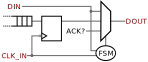
\includegraphics[width=\textwidth]{img/logical}
    \caption{\textbf{Logical Model.} \textmd{
        The Finite State Machine selects between the three modes a node can be
        in. Top: {\em forwarding}, Mid: {\em transmitting}, Bot: {\em
        acknowledging}. This model omits some of the subtleties of
        arbitration,
        see~\ref{sec:state-arbitrate}~\nameref{sec:state-arbitrate} for
        details.
    }}
    \label{fig:logical}
  \end{minipage}
\end{figure}

\begin{figure}[h]
  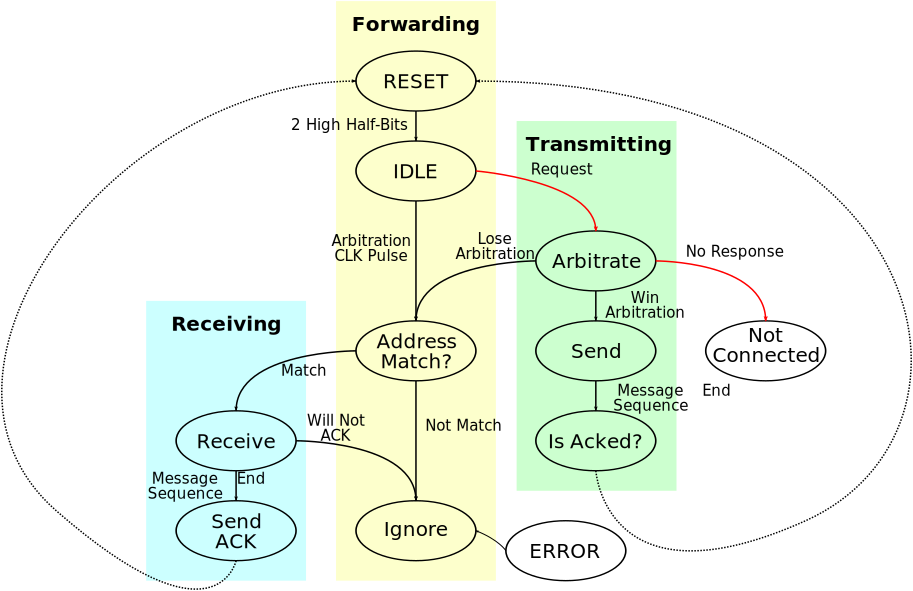
\includegraphics[width=\linewidth]{img/fsm_diagram}
  \caption{\textbf{FSM describing the high-level logical behavior of \bus
    nodes.} \textmd{
    Black arrows indicate transitions that occur on bus clock edges. Not shown
    are implicit arrows from any state to Forwarding.{\sc control}. From any
    {\sc control} state, nodes progress to {\sc idle}.
    }}
\end{figure}

\subsubsection{Forwarding}
Forwarding is the most common state for all \bus nodes. Observe in
\autoref{fig:logical} the very simple, short logic path from {\tt DIN} to
{\tt DOUT}. Nodes are obligated to forward data in less than 10~ns.

\paragraph{Forwarding.\textsc{Idle}}
This is the rest/idle state for \bus nodes. In this state member nodes may be
completely power-gated and asleep. The only obligation is that {\tt DIN} is
forwarded to {\tt DOUT} and {\tt CLKIN} is forwarded to {\tt CLKOUT}.

\medskip
\noindent
{\em Master Node Exception:} In \textsc{idle}, the master node does not
forward {\tt DIN} to {\tt DOUT}.

\paragraph{Forwarding.\textsc{Address\_Match}}
At the start of a new transmission, a forwarding node should monitor the {\tt
DIN} line to see if it is the target for this transmission. If a node matches
its address, it promotes itself from forwarding to receiving. After the first
mis-matched bit a forwarding node transitions to the {\sc ignore} state for
the rest of the transaction.

\paragraph{Forwarding.\textsc{Ignore}}
In {\sc ignore} nodes simply forward data. Nodes remain in this state until
Interrupted. Power-conscious designs may safely power gate everything
except Interrupt detector circuitry while in {\sc ignore}.

\subsubsection{Transmitting}

\paragraph{Transmitting.{\sc arbitrate}}
\label{sec:state-arbitrate}
A node initiates a transmission by pulling its {\tt DOUT} line low. A node may
only attempt to initiate a transmission while the bus is idle. Care must be
taken in detecting the bus idle state when requesting to transmit. In
particular, a node requesting to transmit must ensure that the {\tt CLK} line
is still high, it is not sufficient to rely on the local state machine still
being in the {\sc idle} state\footnote{To envision the case defended against
here, picture a tall stack of nodes, where the bottom node requests the bus.
The master node pulls {\tt CLK} low in response. Shortly before the master
node pulls {\tt CLK} high, a node at the top of the stack (still in the {\sc
idle} state) elects to transmit. There is not enough time for his {\tt DOUT}
to propagate to the bottom node, however, thus when {\tt CLK} goes high, both
the bottom and top nodes believe they have won the arbitration. Designers must
select a sufficiently long period $t_{long}$ to ensure all signals are stable.
Twice the maximum possible propagation delay (delay for falling {\tt CLK} to
furthest node + furthest node's {\tt DOUT} back to closest node) of the system
should be sufficient.}.

The {\sc arbitrate} state is left when the {\tt CLK} line is pulled high by
the master node. If a member node's {\tt DIN} is high on the rising clock
edge, it has won arbitration. A node that loses arbitration should begin
listening to see if it is the destination node. If the {\tt CLK} line never
goes high---where never is defined as four times the minimum clock speed of
\bus\footnote{\hl{TODO: TBD}}---the node should consider itself as
disconnected.

Details of priority arbitration are omitted here for simplicity.
See~\ref{sec:protocol-arbitration}~\nameref{sec:protocol-arbitration} for
details.

\medskip
\noindent
{\em Master Node Exception:} The master node always wins arbitration. Note
that when this occurs, the master node's {\tt DIN} will be low.

\medskip
\noindent
{\em Master Node Exception:} If a master node pulls its {\tt DOUT} line low
and its {\tt DIN} line never goes low, it should be considered
{\sc Not\_Connected}.

\paragraph{Transmitting.{\sc send}}
During {\sc send}, a transmitting node pushes bits onto the bus as described
in~\ref{sec:protocol-transmission}~\nameref{sec:protocol-transmission}.

A transmitting node completes its transmission by Interrupting
(\ref{sec:protocol-interrupt}~\nameref{sec:protocol-interrupt}) the bus and
indicating the transmission is complete.

\paragraph{Transmitting.{\sc control}}
As a transmitter, a node is responsible for the first control bit. This bit
should be set by a transmitter to indicate that the complete message has been
sent. The transmitter must listen to the subsequent control bits to establish
if the message was acknowledged and if the targeted layer is sending a
response.

\subsubsection{Receiving}

\paragraph{Receiving.{\sc Receive}}
A receiving node is also obligated to forward data along the bus. In the
sketch shown in \cref{fig:logical}, during the receiving process, a
receiving node remains in pass-thru mode until Interrupted.

\paragraph{Receiving.{\sc control}}
A receiver must acknowledge the successful receipt of a transmission. If a
receiver wishes to NAK a transmission, it simply does nothing during the
ACK/NAK control bit.

A receiver may also possibly enter control by electing to Interrupt the bus
itself. A receiver will Interrupt a transmission to indicate that its RX
buffer has been overrun and the current transmission must be aborted.

\subsubsection{Exception States}

\paragraph{Exception.{\sc Not\_Connected}}
A robust implementation should include detection of some kind for an attempt
to utilize the bus when the node is not actually connected to a bus (so that
it may report failure). After a node pulls its {\tt DOUT} low there is a
maximum possible $t_{long}$ of \hl{TODO} before a master node must pull
{\tt CLK} low in response. If {\tt CLK} is not pulled low, the node should
consider itself disconnected and report failure to send as appropriate.

\clearpage

\svnInfo $Id$

\section{Bus Design}
\label{sec:protocol}
During normal operation, \bus remains in Bus~Idle~(\ref{sec:protocol-idle}).
A transmission begins with Arbitration~(\ref{sec:protocol-arbitration}), then
Message Transmission~(\ref{sec:protocol-transmission}). The transmitter then
Interrupts~(\ref{sec:protocol-interrupt}) the bus and indicates the complete
message was sent. During the Control~(\ref{sec:protocol-control}) period
acknowledgement is negotiated. After Control, \bus returns to Idle or may
optionally send a response message.

\begin{figure}[h!]
  \figTimingArbitration
\end{figure}

\subsection{Bus~Idle}
\label{sec:protocol-idle}
In \bus Bus~Idle, all lines (clock and data) are high. All member nodes are in
forwarding state and the control node is waiting to begin arbitration.

\subsection{Arbitration}
\label{sec:protocol-arbitration}
To begin arbitration, the bus must be in idle state.

To request to transmit on the bus, a node should pull its {\tt DOUT} line low.
All member nodes remain in forwarding state during arbitration, thus when
their {\tt DIN} line goes low, they are obligated to pull their {\tt DOUT}
line low. The control node, however, does {\bf NOT} pull its {\tt DOUT} line
low in response to its {\tt DIN} line going low. The control node only pulls
its {\tt DOUT} line low when it wishes to transmit on the bus. When the
control node's {\tt DIN} line goes low, it will pull the {\tt CLK} line low
and hold it low for some period $t_{long}$. During {\sc idle} (and thus
arbitration), member nodes must forward the clock signal.

By the end of the period $t_{long}$, the effect of the arbitration is
achieved. A member node is in one of three possible states:
\begin{enumerate}
  \item Clock low, {\tt DIN} high, {\tt DOUT} high -- Lost arbitration
    (didn't participate)
  \item Clock low, {\tt DIN} high, {\tt DOUT} low -- Won arbitration
  \item Clock low, {\tt DIN} low, {\tt DOUT} low -- Lost arbitration
    (either lost, or didn't participate)
\end{enumerate}
If the control node wishes to transmit on the bus, all member nodes will be in
the third state. Note this arbitration protocol introduces a {\em
topology-dependent priority}. Firstly, the control node has a greater priority
than any member node as its {\tt DOUT} will propagate around the entire data
loop. The priority of the member nodes is inversely related to their proximity
to the control node in the data loop. That is, the furthest node from the
control node, the node whose {\tt DIN} is connected to the control node's
{\tt DOUT}, has the highest priority of member nodes. The closest node to the
control node, the node whose {\tt DOUT} is connected to the control node's
{\tt DIN}, has the lowest priority.

At the end of $t_{long}$, the control node drives the {\tt CLK} line high. The
normal arbitration phase ends on this rising edge. The next two clock edges
allow for a high-priority arbitration. As \bus priority is topology-dependent,
we provide a priority arbitration cycle to allow a low priority member node to
preempt transmissions. This priority mechanism is still topology-dependent,
that is, if Node~1 in Figure~\ref{fig:transmission} had also attempted to send
a priority message, it would have won that arbitration as well. The priority
arbitration cycle is two clock edges, the first edge is for nodes to drive
their priority requests onto the bus and the second is to latch the results.
During priority arbitration, the node that won the original arbitration should
{\bf not} forward its {\tt DIN} to {\tt DOUT}. At the end of priority
arbitration, if the original winner did not request a priority message, the
node must sample its {\tt DIN} line. If the line is still low there was no
priority message, if the {\tt DIN} line has gone high, however, the node
must back off and allow the priority message requester to transmit.

Whichever node ultimately won arbitration transitions from a forwarding node
to a transmitting node.

\begin{figure}
  \figTimingInterrupt
\end{figure}
% Footnote tied to \figTimingInterrupt
\footnotetext{This detection must occur on the falling edge since the control
layer requires an edge to sample on and it is sampling its {\tt CLK\_IN} pin
detecting when it is not high. A simple detector can sample this every edge
asserting a signal which is sampled by the controller's FSM at time 8,
transitioning the controller into interrupt mode.}

\subsection{Message Transmission}
\label{sec:protocol-transmission}
The first edge after arbitration is defined as ``Begin~Transmission''. On this
edge, the transmitting node should switch its {\tt DOUT} mux from forwarding
{\tt DIN} to the transmit FIFO. Data is expected to be valid and stable during
every subsequent clock edge.

The first sequence of bits pushed onto \bus are the {\em address} bits. All
nodes on a \bus should listen until their address:
\begin{itemize}
  \item Matches: Node promotes itself from Forwarding.{\sc address\_match} to
    Receiving.{\sc receive}.
  \item Does Not Match: Node transitions from Forwarding.{\sc address\_match}
    to Forwarding.{\sc Ignore}.
\end{itemize}

There is no protocol-level delineation between address and data bits. The
transmitting node sends address$+$data as a continuous stream of bits (for
details on \bus addressing,
see~\ref{sec:spec-address}~\nameref{sec:spec-address}). Once a transmitter has
sent the complete transmission it Interrupts the bus.

\subsection{Interrupt}
\label{sec:protocol-interrupt}
Any node may interrupt \bus at any point mid-transmission. A \bus interrupt is
defined as a series of pulses on the data line with no corresponding clock
edges. After $N$~pulses where $N \ge 3$, a node enters Interrupt\footnote{
  While two pulses is sufficient to distinguish an Interrupt from normal data
  transmission, three pulses provides protection against spurious entry to
  Interrupt from a glitch on data lines.}.

The first rising clock edge after Interrupt is defined as ``Begin~Control''.
The next two clock edges define the control bits.

\subsubsection{Nesting Interrupts}
In normal operation, interrupts are not permitted to ``nest'', that is, the
bus may not be interrupted during the control bits. If an Interrupt sequence
occurs during an existing Interrupt (which may only occur if the bus is being
``rescued'' from some erroneous state), the new interrupt {\bf must} present
control bits {\tt 00}. Any operations requested from the previous Interrupt
state are aborted and the net Interrupt result is {\tt 00}~(General~Error).

\subsection{Control Bits}
\label{sec:protocol-control}

\begin{figure}
  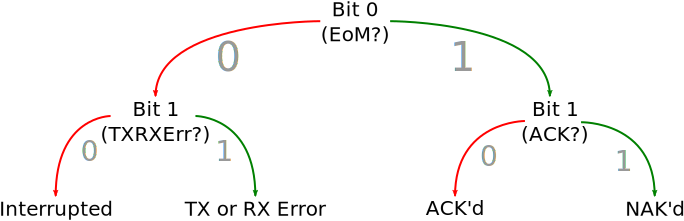
\includegraphics[width=\linewidth]{img/control_bits}
  \caption{After an Interrupt, two control bits follow. The first bit is
    always set by the interrupter and indicates whether the Interrupt was to
    signal the end of message (EoM). If the EoM bit is high, the receiving
    node is responsible for driving the second bit to acknowledge the message.
    If the EoM bit is low, the interrupter is responsible for driving the
    second bit. The TX/RX~Error (TRE) bit is set when a transmitting or
    receiving node encounters an error.
  }
  \label{fig:control-bits}
\end{figure}

The two bits after an Interrupt are defined as Control~Bits.
Figure~\ref{fig:control-bits} is a flowchart indicating the semantic meaning
of the control bits and the resulting state. The first control bit is
unconditionally driven by the interrupting node. If a transmitting node has
interrupted to indicate the end of transmission, it will put a {\tt 1} on the
bus for the first control bit. In all other cases the interrupter must drive
{\tt 0} for the first control bit.

If the first control bit was {\tt 1} then the addressed receiver is
responsible for driving the control bit. If the transmission was sent to the
broadcast address~(\ref{sec:control-broadcast}), all nodes---excluding the
transmitter which forwards---should drive the second control bit low to
acknowledge. The semantic provided to the transmitter of a broadcast message
then is either (1) no nodes received the message or (0) {\em at least} one
node received the message.

If instead the first control bit was {\tt 0} then the interrupter is
responsible for driving the second control bit. If the interrupter is the
transmitter or receiver {\bf and} the issue is related to the current
transmission (e.g. receiver buffer overflow) then the second bit should be set
high. If the purpose of the interruption is unrelated to the current
transmission (e.g. a high-priority, time-critical message) then the second bit
should be set low.

Unless the interruption carries a specific meaning as outlined in this
section, the {\sc 00: Interrupted} state should be used for general or
unclassified interruptions as it carriers the least semantic meaning

\subsection{Return to Idle}
After latching the final Control~Bit (time~20 in
Figure~\ref{fig:interrupt}), one final edge (time~22) is generated to formally
enter {\sc idle}. If, however, the data line is low at this edge, then it
shall be considered the start of a new arbitration cycle instead. The control
node will pull the clock low again in response and begin waiting for
$t_{long}$.

By providing this edge, \bus enables member nodes with absolutely no sense of
time the ability to receive, react to, and respond to messages (albeit with
tight timing constraints).

\begin{quote}
\textit{M3 Implementation Note:} (Referring to
Figure~\ref{fig:interrupt}) A broadcast sleep message cannot be considered a
sleep until time~18 when the transmitter asserts that all the sent bits were
desired to be sent. This leaves edges at time~20 and time~22 as the required
two edges to power gate the layer.

This could be complicated, however, if a node elects (for some reason) to send
a response to the broadcast sleep message. The sleep controller will still
have four edges (Arbitration, Priority~Drive, Priority~Latch,
Begin~Transmission) to wake its bus controller, but the timing between arming
its {\tt CLK\_IN} fall detector and the control node pulling {\tt CLK\_IN} low
in response could cause the sleep controller to miss wakeup.
\end{quote}

\clearpage

\svnInfo $Id$

\section{Specifications}
\label{sec:spec}

\subsection{Granularity}
\label{sec:spec-granularity}
\bus sends data in units of 8~bit bytes. Transmissions must be modulo~8 bits
in length, that is they must end on byte boundaries (for rationale,
see~\nameref{sec:design-granularity}).

\subsection{Endianness: Byte-Level}
\bus sends from Byte 0{\ldots}Byte N.

\subsection{Endianness: Bit-Level}
\bus sends bytes most significant bit first (bit 7{\ldots}0).

\subsection{Minimum Message Length}
The minimum legal message on \bus is {\em zero}~bits long. A zero length
message can be used to query whether a device is present on the bus. A node
receiving a zero length message addressed to it {\bf must} ACK the message.
Whether higher layers are indicated of a query message is implementation
dependent.

See~\ref{sec:spec-interrupt}~\nameref{sec:spec-interrupt} for details on the
minimum uninterruptable message length.

\subsection{Minimum Maximum Message Length}
All \bus control nodes must permit a minimum of 1~K (1024~bits) of data to be
transmitted before aborting a transaction due to a hung transmitter.

The message length counter shall count the number of positive clock edges
received after Begin~Transmission at the control node's {\tt CLK\_IN} port up
to and including the last bit latched (Request~Interrupt in
Figure~\ref{fig:interrupt}). The counter shall be an {\em inclusive} counter,
that is the control node shall not Interrupt until it receives the $N+1$th
bit.

Commands to query and configure the upper bound are specified in
\nameref{sec:channel-2}.

\subsection{Retransmission}
There is no hardware re-transmission primitive. The hardware provides a
transaction-level message acknowledgement, indicating whether the complete
message was received or not. Retransmission of failed messages is left to
software.

\subsection{Minimum Buffer Size}
All \bus nodes are required to support both short and full
addresses~(\ref{sec:spec-address}~\nameref{sec:spec-address}). All \bus nodes
are further required to accept a minimum of 32~bits (4~bytes) of data in an
individual transmission.

\subsection{Buffer Overflow / Flow Control}
On the average, the expectation in a \bus system is that a transmitting node
knows the capacity of the receiving node. If a receiving node does not have
enough space for the current transmission, it {\bf must} Interrupt the current
transmission and indicate a receiver error (Control~Bits:~{\tt 01}).

The receiver must Interrupt as soon as it is {\em certain} that it has
exceeded its receive capacity. This detection must be performed carefully and
must take into account that two bits beyond the complete transmission may be
temporarily received (as is the case for Node~1 in
Figure~\ref{fig:interrupt}). The receiving state machine should not transition
into {\sc decided\_to\_interrupt} until the \nth{3}~bit of a byte that it does
not have space for. The receiver may wait until the \nth{8}~bit to transition
its state machine to request interrupt, but no later than that such that it is
assured that it will interrupt the transmission before the transmitter
attempts to interrupt to signal end of message even if the receiver is of
lower priority.
% XXX This should be a testbench.. all the specs -> tb's?

\subsection{Clock Speed}
\hl{TODO: What is appropriate specification for clock speeds?} I2C has defined
`speed-classes'; SPI is a free-for-all; UART \& co has bauds...

\subsection{Addressing}
\label{sec:spec-address}
\bus defines two types of addresses: \textit{short} 8-bit addresses and
\textit{full} 32~bit addresses. No short address may begin with {\tt 1111} and
all full addresses must begin with {\tt 1111}. Address assignment is laid out
in~\ref{sec:addressing-short}~\nameref{sec:addressing-short}
and~\ref{sec:addressing-full}~\nameref{sec:addressing-full} respectively.
%
Addresses {\tt 0x00}, {\tt 0x01}, and {\tt 0xffffffff} are reserved. Their
function is detailed in~\ref{sec:control}~\nameref{sec:control}.

\subsection{Unassigned Short Prefix: \texttt{0b1111}}
\label{sec:spec-unassigned-short-prefix}
Out of reset, nodes self-assign a short prefix of {\tt 0b1111}. This short
prefix shall be considered as a sentinel value where short prefixes are
reported, indicating that the node does not currently have a short prefix
assigned.

\subsection{Interrupt Rules}
\label{sec:spec-interrupt}
\bus permits any node to interrupt any message for any reason. To allow for
minimal forward progress, however, \bus requires that nodes permit a minimum
of 32~bits (4~bytes) be transmitted without interruption. An exception is made
for the transmitting node, which is permitted to send messages shorter than
32~bits.

Nodes wishing to interrupt must wait until either 41 or 65 clocks after
Begin~Transmission to interrupt the bus (depending on whether the current
message was addressed to a short address or full address). The interrupting
node must wait until it has latched the \nth{33} bit of data before attempting
to interrupt\footnote{
  If the node instead attempted to interrupt on the \nth{32} bit and was a
  topologically higher-priority node, it would override the transmitter during
  Interrupt priority arbitration, not permitting the transmitter to signal
  End~of~Message.}.

\subsection{Failed Arbitration (Spurious Wakeup)}
\label{sec:spec-spurious}
During normal arbitration, when the arbitration is resolved the control node's
{\tt DIN} line should be low no matter who is participating. If the control
node finds its {\tt DIN} line is high on the arbitration edge, it would
indicate that no one is participating. The control node must treat this as an
error and reset the bus.

The control node {\bf must not} immediately interrupt the bus, however. As
laid out in~\ref{sec:design-power-gated}~\nameref{sec:design-power-gated}, the
arbitration edges may be used as input to node sleep controllers. To avoid
potential issues related to half-waking power gated nodes, the control node
must wait until Begin~Transmission (that is, have generated four clock edges)
before interrupting the bus.

The control bits {\bf must} be driven by the control layer. They {\bf must} be
{\tt 00}, general error.

\clearpage

\svnInfo $Id$

\section{ToDo}
\label{sec:todo}

\subsection{Future Extensions}
\label{sec:todo-extensions}
There are properties that would be nice to have, but introduce greater
complexity. While they are not in the current design, some methods for
designing them are considered here such that they are still feasible for
future implementation in a backwards-compatible manner.

\subsubsection{Automatically fragment long \proto messages}
Add a configuration register for a maximum message length, maybe one for each
message type, that limits maximum transaction length. Requests to send
messages over this length should be automatically fragmented by the sender.

\subsubsection{Full Address Support in \proto}
\label{sec:todo-full-addr}
Currently there is no way to generate a response that sends a message to a
full address. A full prefix is 24~bits long. The following are some possible
methods to support full addresses:
\begin{enumerate}
  \item {\bf Use new FU\_IDs.} Easiest solution, but uses a lot of the
    remaining FU\_IDs. Could do something creative such as the full prefix
    (24~bits) is sent and then the next 3~or 4~bits map the remaining words
    onto one of the existing FU\_IDs. This wastes at least the 4~bits that
    previously specified the short prefix.
  \item {\bf Full Prefix Register(s).} Store a full prefix in a register.
    Since registers are also 24~bits, they can hold a full prefix exactly.
    This is actually a little unfortunate, since a destination FU\_ID also
    needs to be specified. While the short prefix {\tt 1111} in the current
    message can be used as a sentinel, something needs to indicate which
    register the full prefix should be read from. The FU\_ID field could be
    repurposed to this end, but then there is nothing to specify the FU\_ID of
    the eventual message. This could spill over to two registers, but that is
    an inefficient use of registers. Full prefix registers also become another
    contested, shared resource with this scheme.
  \item {\bf Optional Extra Word.} Use the existing short prefix as a
    sentinel. If set to {\tt 1111}, the (next, last) word will be the full
    prefix. Since the short prefix is the first 4~bits, could also just
    ``replace'' the first word of the message with a full address---this has
    nice symmetry with how short/full prefixes are interpreted on the bus. In
    any of these cases, an extra 8~bits become available for some other
    purpose. The runtime variable length message can be tricky to implement.
    Injecting an extra word into the middle of a message makes it harder for
    simple devices with fixed send buffers to support these messages.
\end{enumerate}

\subsubsection{Finer-grained DMA control}
\label{sec:todo-fine-grain-dma}
Currently DMA is all-or-nothing. This is how pretty much all M0 DMA
controllers work, but it's not the best. It would be neat to explore an IOMPU
concept (analagous to A-series IOMMUs). Another option could be to pass the
request to the core as an interrupt, but I actually think that's more
complicated.


\subsubsection{Reg \#240: Register Message Control}
\label{cmd:conf-reg-ctrl}

\begin{bytefield}{8}
  \bitheader{0-7} \\
  \colorbitbox{lightgreen}{2}{11}
  \colorbitbox{lightergreen}{6}{110000}
\end{bytefield}
~
\begin{bytefield}{24}
  \bitheader{0-23} \\
  \bitbox{1}{\begin{sideways}{\tiny EN}\end{sideways}}
  \colorbitbox{lightgray}{23}{Reserved}
\end{bytefield}
\hfill\textbf{Default: \texttt{0x800000}}
\\

\begin{itemize}
  \item {\tt \{R[23]\}: Enable (EN).}
    \subitem Controls whether register writes to this device are enabled. If
    {\tt EN} is {\tt 0}, attempts to write registers~\#0--247 are silently
    ignored.
    \subitem {\bf Note:} Registers~\#248--255 ({\tt b'11111XXX}) can always be
    written.
    \subitem {\bf Acknowledement/Interjection:} Since a single register write
    transaction could write both enabled and disabled registers, a node should
    not interject when a disabled register is written. A node should ACK to
    indicate that the transmission was received successfully, even if nothing
    is actually written.
    {\em This behavior is subject to change in future revisions of \proto.}
    \subitem {\color{red} \bf Warning:} If {\tt EN} is disabled, it cannot be
    re-enabled by a write to this register since register writes are disabled.
    Access can be recovered using \nameref{cmd:conf-reg-reset}, however this
    will reset all registers.
    \subitem \hl{TODO} What about a local write (e.g. a register write via an
    interrupt from the CPU)? Should probably always allow those. Does that
    make sense as an exception?
\end{itemize}


%%%%%%%%%%%%%%%%%%%%%%%%%%%%%%%%%%%%
\clearpage
\section{Document Revision History}
\label{sec:revisions}

\begin{itemize}

\item Revision 0.5 {\footnotesize(r2986)} -- Feb 10, 2012
\subitem Overhaul reset design
\subitem Upgrade RX overflow Reset to requirement from optional optimization

\item Revision 0.4 {\footnotesize(r2850)} -- Jan 22, 2012
\subitem Begin to address Reset issues

\item Revision 0.3 {\footnotesize(r2746)} -- Jan 10, 2012
\subitem Commit to 4-pulse design, update accordingly
\subitem Add TODO section of new considerations / issues

\item Revision 0.2 {\footnotesize(r2697)} -- Jan 5, 2012
\subitem Add skeleton of design considerations / requirements
\subitem Add discussion of \bus states, state diagram
\subitem Several clarifications

\item Revision 0.1 {\footnotesize(r2653)} -- Dec 19, 2012
\subitem Initial revision

\end{itemize}

%%%%%%%%%%%%%%%%%%%%%%%%%%%%%%%%%%%%
\clearpage
\appendix
\section{Other MES, ACK, RST Designs}
\label{sec:appendix-reset}
% \svnInfo $Id$

\subsection{MES 0110, ACK 0110, RST 010}

\subsubsection{$1\phi$ Offset}

\begin{figure}
\begin{subfigure}{\textwidth}
    \centering
    \huge {\bf MES 0110, ACK 0110, RST 01011 Broken:}

    \tiny
    \begin{tikztimingtable}[timing/slope=.3,timing/wscale=1.0]
      Din  & L0.8L4{4L}4{4H}2{4L}0.2LLLXXHHH4H    0.5H8{2L}8{2H}8{2L}7{2H}1.5HH \\
      Dout & L0.0L4{4L}4{4H}2{4L}   LLLXXHHH4H    0.5H8{2L}8{2H}8{2L}7{2H}1.5HH \\
      ~~~~ & D{}{16D{Data 0}}{16D{Data 1}}{12D{Data 0}}{44D{Error (Forwarding)}}{28D{Reset}}D
      \\
      \\
      Din  & L3{4L}LLLXXHHH2{4H}HHHXXLLL{4L}{4L}.5L.5HHHH4H    0.8H8{2L}8{2H}8{2L}7{2H}1.2HH \\
      Dout & L3{4L}LLLXXHHH2{4H}HHHXXLLL2{4L}2{4H} HLLL8H4LLH8{2H}8{2L}7{2H}H \\
      ~~~~ & {5D{Data 0}}{32D{End Sequence}}{28D{Acknowledgement Attempt}}{32D{Error (Forwarding)}}{20D{Reset}}D \\
      %\\
      Din  & L0.5L4{4L}4{4H}3{4L}{4H}3.5H HLLL8H4LLH8{2H}8{2L}7{2H}H \\
      Dout & L0.5L4{4L}4{4H}3{4L}{4H}3.5H 8{2L}8{2H}8{2L}7{2H}2.0HH \\
      CLK  & C26{2C}4L15{4C}H \\
      \extracode
        \begin{pgfonlayer}{background}
          \begin{scope}[semitransparent,dashed]
            \vertlines{1,9,...,49}
            \pgfmathparse{\twidth-4}
            \vertlines{57,65,...,\pgfmathresult}
            \vertlines[color=red]{5,13,...,49}
            \vertlines[color=blue]{53,61,...,\pgfmathresult}
            \pgfmathparse{\twidth-1}
            \vertlines{\pgfmathresult}
          \end{scope}
          \begin{scope}[thick]
            \draw[red]   (17,-4.5)  ellipse (2 and 4);
            \draw[green] (33,-4.5)  ellipse (2 and 4);
            \draw[blue]  (47,-13.5) ellipse (3 and 1.25);
          \end{scope}
          \begin{scope}[semitransparent]
            % TX
            \filldraw[yellow]    ( 1,-0.5) rectangle ( 5,-2.5);
            \filldraw[yellow]    (17,-0.5) rectangle (21,-2.5);
            \filldraw[yellow]    (33,-0.5) rectangle (37,-2.5);
            % RX
            \filldraw[yellow]    (37,-8.5) rectangle (41,-10.5);
            \filldraw[yellow]    (45,-8.5) rectangle (49,-10.5);
            \filldraw[yellow]    (57,-8.5) rectangle (65,-10.5);
            % CLK
            \filldraw[yellow]    ( 1,-16.5) rectangle (53,-18.5);
            \filldraw[cyan,opacity=.25] (53,-14.5) rectangle (\twidth-1, -18.5);
          \end{scope}
          \foreach \n [evaluate=\n as \l using int((\n-1)/4)] in {1,5,...,\twidth}
            \draw (\n,-19) -- +(0,-.2)
              node [below,inner sep=2pt] {\scalebox{.75}{\tiny\l}};
        \end{pgfonlayer}
        \begin{scope}
          [font=\sffamily\small,shift={(-3.0em,-0.5)},anchor=east,color=blue]
          \node at (  0,   0) {TX};
          \node at (  0,  -8) {RX};
          \node at (  0, -15) {Ctl};
        \end{scope}
        \begin{scope}
          [font=\sc\tiny,anchor=north,shift={(0,3em)},color=brown]
          \foreach \x [evaluate=\x] in {1,17,...,47}
            \foreach \offset/\l in {0/Drive1,4/Latch1,8/Drive2,12/Latch2}
              \node [rotate=45] at (\x+\offset,0) {\l};
          \node [rotate=45] at (49,0) {Drive1};
          \def\base{57}
          \node [rotate=45] at (\base+0, 0)  {Latch1};
          \node [rotate=45] at (\base+8, 0)  {Drive2};
          \node [rotate=45] at (\base+16, 0) {Latch2};
          \node [rotate=45] at (\base+24, 0) {Drive1};
          \node [rotate=45] at (\base+32, 0) {Latch1};
          \node [rotate=45] at (\base+40, 0) {Reset};
          \node [rotate=45] at (\base+48, 0) {Reset};
          \node [rotate=45] at (\base+56, 0) {Reset};
        \end{scope}
        \begin{scope}
          [font=\bf\tiny,anchor=north,shift={(.2,-3.1em)},color=red]
          \foreach \x [evaluate=\x] in {1,17,...,47}
            \foreach \offset/\l in {0/L2,4/D1,8/L1,12/D2}
              \node [rotate=45] at (\x+\offset,0) {\l};
          \node [rotate=45] at (49,0) {L2};
          \def\base{57}
          \node [rotate=45] at (\base+0, 0)  {D1};
          \node [rotate=45] at (\base+8, 0)  {L1};
          \node [rotate=45] at (\base+16, 0) {D2};
          \node [rotate=45] at (\base+24, 0) {L2};
          \node [rotate=45] at (\base+32, 0) {D1};
          \node [rotate=45] at (\base+40, 0) {L1};
          \node [rotate=45,color=brown] at (\base+48, 0) {R};
          \node [rotate=45,color=brown] at (\base+56, 0) {R};
        \end{scope}
        \begin{scope}
          [font=\sc\tiny,anchor=north,shift={(0,3em)},color=blue]
          \def\base{53}
          \node [rotate=45] at (\base, 0) {Reset-S0-D};
          \node [rotate=45] at (\base+8, 0) {Reset-S0-L};
          \node [rotate=45] at (\base+16, 0) {Reset-S1-D};
          \node [rotate=45] at (\base+24, 0) {Reset-S1-L};
          \node [rotate=45] at (\base+32, 0) {Reset-S0-D};
          \node [rotate=45] at (\base+40, 0) {Reset-S0-L};
          \node [rotate=45] at (\base+48, 0) {Reset-R-D};
          \node [rotate=45] at (\base+56, 0) {Reset-R-L};
          \node [rotate=45,color=black] at (\base+64, 0) {Idle};
        \end{scope}
    \end{tikztimingtable}
    \caption{Transmitter is sending data bits 0, 1, 0 ({\tt 001100}). The
transmitter latches the receiving layer's high bit during {\sc latch2} at time
11, aborts its transmission, and begins forwarding. At time 16, the RX layer
latches a {\tt 0} when it had attempted to drive a {\tt 1}, and aborts the
transmission.}

    \begin{tikztimingtable}[timing/slope=.3]
      Din  & L0.8L4{4L}4{4H}2{4L}0.2LLLXXHHH4H     0.5H8{2L}8{2H}8{2L}7{2H}1.5HH \\
      Dout & L0.0L4{4L}4{4H}2{4L}   LLLXXHHH4U    4U.5L6{2L}8{2H}8{2L}7{2H}1.5HH \\
      ~~~~ & D{}{16D{Data 0}}{16D{Data 1}}{16D{Data 0}}{24D{Data X}}{16D{Error (Forwarding)}}{28D{Reset}}D
      \\
      \\
      Din  & L3{4L}LLLXXHHH2{4H}HHHXXLLL{4L}{4L}.5L.5HHHH4X 4X0.8X 6{2L}    8{2H}8{2L}7{2H}1.2HH \\
      Dout & L3{4L}LLLXXHHH2{4H}HHHXXLLL2{4L}{4H}4X         4X4{2H}2{2L}0.8L8{2H}8{2L}7{2H}1.2HH\\
      ~~~~ & {5D{Data 0}}{32D{End Sequence}}{28D{Acknowledgement}}{32D{Error (Forwarding)}}{20D{Reset}}D \\
      %\\
      Din  & L0.5L4{4L}4{4H}3{4L}{4H}4X   4X4{2H}2{2L}8{2H}8{2L}7{2H}1.5HH  \\
      Dout & L0.5L4{4L}4{4H}3{4L}{4H}3.5H     8{2L}8{2H}8{2L}7{2H}2.0HH \\
      CLK  & C26{2C}4L15{4C}H \\
      \extracode
        \begin{pgfonlayer}{background}
          \begin{scope}[semitransparent,dashed]
            \vertlines{1,9,...,49}
            \pgfmathparse{\twidth-4}
            \vertlines{57,65,...,\pgfmathresult}
            \vertlines[color=red]{5,13,...,49}
            \vertlines[color=blue]{53,61,...,\pgfmathresult}
            \pgfmathparse{\twidth-1}
            \vertlines{\pgfmathresult}
          \end{scope}
          \begin{scope}[thick]
            \draw[red]   (17,-4.5)  ellipse (2 and 4);
            \draw[green] (33,-4.5)  ellipse (2 and 4);
            \draw[blue]  (47,-13.5) ellipse (3 and 1.25);
          \end{scope}
          \begin{scope}[semitransparent]
            % TX
            \filldraw[yellow]    ( 1,-0.5) rectangle ( 5,-2.5);
            \filldraw[yellow]    (17,-0.5) rectangle (21,-2.5);
            \filldraw[yellow]    (33,-0.5) rectangle (37,-2.5);
            \filldraw[yellow]    (49,-0.5) rectangle (57,-2.5);
            % RX
            \filldraw[yellow]    (37,-8.5) rectangle (41,-10.5);
            \filldraw[yellow]    (45,-8.5) rectangle (49,-10.5);
            \filldraw[yellow]    (57,-8.5) rectangle (65,-10.5);
            % CLK
            \filldraw[yellow]    ( 1,-16.5) rectangle (53,-18.5);
            \filldraw[cyan,opacity=.25] (53,-14.5) rectangle (\twidth-1, -18.5);
          \end{scope}
          \foreach \n [evaluate=\n as \l using int((\n-1)/4)] in {1,5,...,\twidth}
            \draw (\n,-19) -- +(0,-.2)
              node [below,inner sep=2pt] {\scalebox{.75}{\tiny\l}};
        \end{pgfonlayer}
        \begin{scope}
          [font=\sffamily\small,shift={(-3.0em,-0.5)},anchor=east,color=blue]
          \node at (  0,   0) {TX};
          \node at (  0,  -8) {RX};
          \node at (  0, -15) {Ctl};
        \end{scope}
        \begin{scope}
          [font=\sc\tiny,anchor=north,shift={(0,3em)},color=brown]
          \foreach \x [evaluate=\x] in {1,17,...,47}
            \foreach \offset/\l in {0/Drive1,4/Latch1,8/Drive2,12/Latch2}
              \node [rotate=45] at (\x+\offset,0) {\l};
          \node [rotate=45] at (49,0) {Drive1};
          \def\base{57}
          \node [rotate=45] at (\base+0, 0)  {Latch1};
          \node [rotate=45] at (\base+8, 0)  {Drive2};
          \node [rotate=45] at (\base+16, 0) {Latch2};
          \node [rotate=45] at (\base+24, 0) {Drive1};
          \node [rotate=45] at (\base+32, 0) {Latch1};
          \node [rotate=45] at (\base+40, 0) {Reset};
          \node [rotate=45] at (\base+48, 0) {Reset};
          \node [rotate=45] at (\base+56, 0) {Reset};
        \end{scope}
        \begin{scope}
          [font=\bf\tiny,anchor=north,shift={(.2,-3.1em)},color=red]
          \foreach \x [evaluate=\x] in {1,17,...,47}
            \foreach \offset/\l in {0/L2,4/D1,8/L1,12/D2}
              \node [rotate=45] at (\x+\offset,0) {\l};
          \node [rotate=45] at (49,0) {L2};
          \def\base{57}
          \node [rotate=45] at (\base+0, 0)  {D1};
          \node [rotate=45] at (\base+8, 0)  {L1};
          \node [rotate=45] at (\base+16, 0) {D2};
          \node [rotate=45] at (\base+24, 0) {L2};
          \node [rotate=45] at (\base+32, 0) {D1};
          \node [rotate=45] at (\base+40, 0) {L1};
          \node [rotate=45,color=brown] at (\base+48, 0) {R};
          \node [rotate=45,color=brown] at (\base+56, 0) {R};
        \end{scope}
        \begin{scope}
          [font=\sc\tiny,anchor=north,shift={(0,3em)},color=blue]
          \def\base{53}
          \node [rotate=45] at (\base, 0) {Reset-S0-D};
          \node [rotate=45] at (\base+8, 0) {Reset-S0-L};
          \node [rotate=45] at (\base+16, 0) {Reset-S1-D};
          \node [rotate=45] at (\base+24, 0) {Reset-S1-L};
          \node [rotate=45] at (\base+32, 0) {Reset-S0-D};
          \node [rotate=45] at (\base+40, 0) {Reset-S0-L};
          \node [rotate=45] at (\base+48, 0) {Reset-R-D};
          \node [rotate=45] at (\base+56, 0) {Reset-R-L};
          \node [rotate=45,color=black] at (\base+64, 0) {Idle};
        \end{scope}
    \end{tikztimingtable}
    \caption{Transmitter is sending data bits 0, 1, 0 ({\tt 001100}). The
transmitter latches {\tt 0} at time 11 and does not yet know there is an
issue. At time 12, so long as the transmitter is sending another full bit
it does not matter whether that bit is a {\tt 0} or {\tt 1} as the control
layer's reset will propagate during the {\sc latch1}, {\sc drive2}, and {\sc
latch2} states.  Shown here is the assumption that the RX node latches the
previous {\tt 1} at time 12. If it had latched {\tt 0} instead it would enter
Reset at time 12.}


    \begin{tikztimingtable}[timing/slope=.3]
      Din  & L0.8L4{4L}4{4H}{4L}{4L}{4H}{4H}{4H}{4H}{4L}{4L}{16L} \\
      Dout & L0.0L4{4L}4{4H}{4L}{4L}{4H}{4H}{4H}{4H}{4L}{4L}{16L}\\
      ~~~~ & D{}{16D{Data 0}}{16D{Data 1}}{8D{MES 0}}{8D{MES 1}}{8D{MES 1}}{8D{MES 0}}{8D{ACK 0}}{8D{NAK}}
      \\
      \\
      Din  & L3{4L}LLLXXHHH2{4H}HHHXXLLL{3L}XX{3H}{4H}{4H}{3H}XX{3L}{4L}{16L} \\
      Dout & L3{4L}LLLXXHHH2{4H}HHHXXLLL{4L}{4H}{4H}{4H}{4H}X{3L}{4L}{16L} \\
      ~~~~ & {5D{Data 0}}{32D{End Sequence}}{32D{Acknowledgement}}D{} \\
      %\\
      Din  & L0.5L4{4L}4{4H}{4L}{4L}{4H}{4H}{4H}{4H}{4L}{4L}{16L} \\
      Dout & L0.5L4{4L}4{4H}{4L}{4L}{4H}{4H}{4H}{4H}{4L}{4L}{16L} \\
      %CLK  & C26{2C}4L15{4C}H \\
      CLK  & C46{2C}4L \\
      \extracode
        \begin{pgfonlayer}{background}
          \begin{scope}[semitransparent,dashed]
            \vertlines{1,9,...,49}
            \pgfmathparse{\twidth-4}
            \vertlines{57,65,...,\pgfmathresult}
            \vertlines[color=red]{5,13,...,49}
            \vertlines[color=blue]{53,61,...,\pgfmathresult}
            \pgfmathparse{\twidth-1}
            \vertlines{\pgfmathresult}
          \end{scope}
          \begin{scope}[semitransparent]
            % TX
            \filldraw[yellow]    ( 1,-0.5) rectangle ( 5,-2.5);
            \filldraw[yellow]    (17,-0.5) rectangle (21,-2.5);
            \filldraw[yellow]    (33,-0.5) rectangle (37,-2.5);
            \filldraw[yellow]    (41,-0.5) rectangle (45,-2.5);
            \filldraw[yellow]    (49,-0.5) rectangle (53,-2.5);
            \filldraw[yellow]    (57,-0.5) rectangle (61,-2.5);
            % RX
            \filldraw[yellow]    (37,-8.5) rectangle (41,-10.5);
            \filldraw[yellow]    (45,-8.5) rectangle (49,-10.5);
            \filldraw[yellow]    (53,-8.5) rectangle (57,-10.5);
            \filldraw[yellow]    (61,-8.5) rectangle (65,-10.5);
          \end{scope}
        \end{pgfonlayer}
        \begin{scope}
          [font=\sffamily\small,shift={(-3.0em,-0.5)},anchor=east,color=blue]
          \node at (  0,   0) {TX};
          \node at (  0,  -8) {RX};
          \node at (  0, -15) {Ctl};
        \end{scope}
        \begin{scope}
          [font=\sc\tiny,anchor=north,shift={(0,3em)},color=brown]
          \foreach \x [evaluate=\x] in {1,17,...,\twidth}
            \foreach \offset/\l in {0/Drive1,4/Latch1,8/Drive2,12/Latch2}
              \node [rotate=45] at (\x+\offset,0) {\l};
        \end{scope}
        \begin{scope}
          [font=\bf\tiny,anchor=north,shift={(.2,-3.1em)},color=red]
          \foreach \x [evaluate=\x] in {1,17,...,\twidth}
            \foreach \offset/\l in {0/L2,4/D1,8/L1,12/D2}
              \node [rotate=45] at (\x+\offset,0) {\l};
        \end{scope}
        \begin{scope}
          [font=\sc\tiny,anchor=north,shift={(0,3em)},color=blue]
          \def\base{53}
        \end{scope}
    \end{tikztimingtable}
    \caption{Transmitting is sending data bits 0, 1, then
Message~End~Sequence ({\tt 00110110})}
\end{subfigure}
\caption{Detail of a $1\phi$TX~0$\rightarrow$1 error. The top labels are the
current global bus state. The red labels above the RX waveform indicate the
local $1\phi$ state machine. {\tt DOUT} lines are colored to indicate when a
node is driving (yellow), otherwise it is forwarding its {\tt DIN} value.
This scheme fails in the third case (TX 0,1,MES) as the RX node can
incorrectly conclude it has ACK'd a message. While this is detectable by
observing that the ACK is not immediately followed by Reset, this is
cumbersome and not very intuitive.
}
\label{fig:reset-1phi-tx-0-1}
\end{figure}


\FloatBarrier
\clearpage
%\svnInfo $Id$

\section{MES 0111, ACK 1001, RST 010}

\subsection{An Ideal Transmission}
~

\begin{figure}[!h]
\begin{subfigure}{\textwidth}
    \ssmall
    \begin{tikztimingtable}[timing/slope=.3]
      %       |   D1    | D0  | D1  |     MES       |
      Din  & L 1.4L8{2H} 8{2L} 8{2H} 4{2L}11{2H}0.6H H \\
      Dout & L 0.0L8{2H} 8{2L} 8{2H} 4{2L}11{2H}2.0H H \\
      \\
      Din  & L 0.2L8{2H} 8{2L} 8{2H} 4{2L}11{2H}1.8H H \\
      Dout & L 0.4L8{2H} 8{2L} 8{2H} 4{2L}11{2H}1.6H H \\
      \\
      Din  & L 0.6L8{2H} 8{2L} 8{2H} 4{2L}11{2H}1.4H H \\
      Dout & L 0.8L8{2H} 8{2L} 8{2H} 4{2L}11{2H}1.2H H \\
      \\
      Din  & L 1.0L8{2H} 8{2L} 8{2H} 4{2L}11{2H}1.0H H \\
      Dout & L 1.2L8{2H} 8{2L} 8{2H} 4{2L}11{2H}0.8H H \\
      CLK  & C 40{2C}                                C \\
           & \\
      \extracode
        \begin{pgfonlayer}{background}
          \begin{scope}[semitransparent,semithick]
            \vertlines{1,17,...,81}
          \end{scope}
          \begin{scope}[semitransparent,semithick,dashed]
            \vertlines{9,25,...,81}
          \end{scope}
          \begin{scope}[semitransparent,semithick,dashed,color=red]
            \vertlines{5,13,...,81}
          \end{scope}
          \begin{scope}[semitransparent]
            % TX
            \filldraw[yellow] ( 1,-0.5)  rectangle ( 5,-2.5);
            \filldraw[yellow] (17,-0.5)  rectangle (21,-2.5);
            \filldraw[yellow] (33,-0.5)  rectangle (37,-2.5);
            \filldraw[yellow] (49,-0.5)  rectangle (53,-2.5);
            \filldraw[yellow] (57,-0.5)  rectangle (61,-2.5);
            \filldraw[yellow] (65,-0.5)  rectangle (69,-2.5);
            \filldraw[yellow] (73,-0.5)  rectangle (77,-2.5);
            % RX
            \filldraw[yellow] (81,-6.5)  rectangle (82,-8.5);
            % Clk
            \filldraw[yellow] ( 0,-20.5) rectangle (82,-22.5);
          \end{scope}
        \end{pgfonlayer}
        \begin{scope}
          [font=\sffamily\small,shift={(-3.0em,-0.5)},anchor=east,color=blue]
          \node at (  0,   0) {TX};
          \node at (  0,  -6) {RX};
          \node at (  0, -12) {Fwd};
          \node at (  0, -19) {Ctl};
        \end{scope}
        \begin{scope}
          [font=\sc\tiny,anchor=north,shift={(0,3em)},color=brown]
          \foreach \x [evaluate=\x] in {1,17,...,77}
            \foreach \offset/\l in {0/Drive1,4/Latch1,8/Drive2,12/Latch2}
              \node [rotate=45] at (\x+\offset,0) {\l};
          \node[rotate=45] at (81,0) {Drive1};
        \end{scope}
        \begin{scope}
          [font=\small,anchor=south,shift={(1,-18em)}]
          \draw
            (0,0) node[] (a) {}
            (16,0) node[] (c) {}
            (32,0) node[] (e) {}
            (48,0) node[] (g) {}
            (80,0) node[] (i) {}
            (82,0) node[] (z) {\ldots};
          \node[right=4 of a] (b) {Data 1};
          \node[right=4 of c] (d) {Data 0};
          \node[right=4 of e] (f) {Data 1};
          \node[right=8 of g] (h) {End Sequence};
          \draw[->] (b.west) -- (a.east);
          \draw[<-] (c.west) -- (b.east);
          \draw[->] (d.west) -- (c.east);
          \draw[<-] (e.west) -- (d.east);
          \draw[->] (f.west) -- (e.east);
          \draw[<-] (g.west) -- (f.east);
          \draw[->] (h.west) -- (g.east);
          \draw[<-] (i.west) -- (h.east);
          %\draw[<-] (i.east) -- (z.west);
        \end{scope}
    \end{tikztimingtable}

    \begin{tikztimingtable}[timing/slope=.3]
      %       |         ACK           |
      Din  & H 1.0H4{2H}8{2L}3{2H}1.0H 0.2H8{2L}8{2H}8{2L}7{2H}1.8H H \\
      Dout & H 1.2H4{2H}8{2L}3{2H}0.8H 0.4H8{2L}8{2H}8{2L}7{2H}1.6H H \\
      \\
      Din  & H 1.4H4{2H}8{2L}3{2H}0.6H 0.6H8{2L}8{2H}8{2L}7{2H}1.4H H \\
      Dout & H 0.0H4{2H}8{2L}3{2H}2.0H 0.8H8{2L}8{2H}8{2L}7{2H}1.2H H \\
      \\
      Din  & H 0.2H4{2H}8{2L}3{2H}1.8H 1.0H8{2L}8{2H}8{2L}7{2H}1.0H H \\
      Dout & H 0.4H4{2H}8{2L}3{2H}1.6H 1.2H8{2L}8{2H}8{2L}7{2H}0.8H H \\
      \\
      Din  & H 0.6H4{2H}8{2L}3{2H}1.4H 1.4H8{2L}8{2H}8{2L}7{2H}0.6H H \\
      Dout & H 0.8H4{2H}8{2L}3{2H}1.2H 0.0H8{2L}8{2H}8{2L}7{2H}2.0H H \\
      CLK  & C 16{2C}4L15{4C}                                       H \\
      ~~~  & C 47{2C}2H                                             H \\
           & \\
      \extracode
        \begin{pgfonlayer}{background}
          \begin{scope}[semitransparent,semithick]
            \vertlines{1,17,...,32}
            \vertlines{37,53,69}
          \end{scope}
          \begin{scope}[semitransparent,semithick,dashed]
            \vertlines{9,25,...,32}
            \vertlines{97}
          \end{scope}
          \begin{scope}[semitransparent,semithick,dashed,color=red]
            \vertlines{5,13,...,32}
            \vertlines{45,61,77,85,93}
          \end{scope}
          \begin{scope}[semitransparent,semithick,color=blue]
            \vertlines{33,49,...,89}
          \end{scope}
          \begin{scope}[semitransparent,semithick,dashed,color=blue]
            \vertlines{41,57,...,89}
          \end{scope}
          \begin{scope}[semitransparent,yellow]
            % TX
            %\filldraw[yellow] ( 0,-0.5)  rectangle (1,-2.5);
            % RX
            \filldraw ( 1,-6.5)  rectangle ( 5,-8.5);
            \filldraw ( 9,-6.5)  rectangle (13,-8.5);
            \filldraw (17,-6.5)  rectangle (21,-8.5);
            \filldraw (25,-6.5)  rectangle (29,-8.5);
            % Clk
            \filldraw ( 0,-20.5) rectangle (33,-22.5);
          \end{scope}
          \begin{scope}[cyan,opacity=.25]
            \filldraw   (33,-18.5) rectangle (\twidth-1,-22.5);
          \end{scope}
        \end{pgfonlayer}
        \begin{scope}
          [font=\sffamily\small,shift={(-3.0em,-0.5)},anchor=east,color=blue]
          \node at (  0,   0) {TX};
          \node at (  0,  -6) {RX};
          \node at (  0, -12) {Fwd};
          \node at (  0, -19) {Ctl};
        \end{scope}
        \begin{scope}
          [font=\sc\tiny,anchor=north,shift={(0,3em)},color=brown]
          \foreach \x [evaluate=\x] in {1,17,...,29}
            \foreach \offset/\l in {0/Drive1,4/Latch1,8/Drive2,12/Latch2}
              \node [rotate=45] at (\x+\offset,0) {\l};
          \def\base{37}
          \node [rotate=45] at (\base+0, 0) {Drive1};
          \node [rotate=45] at (\base+8, 0) {Latch1};
          \node [rotate=45] at (\base+16, 0) {Drive2};
          \node [rotate=45] at (\base+24, 0) {Latch2};
          \node [rotate=45] at (\base+32, 0) {Drive1};
          \node [rotate=45] at (\base+40, 0) {Latch1};
          \node [rotate=45] at (\base+48, 0) {Reset};
          \node [rotate=45] at (\base+56, 0) {Reset};
        \end{scope}
        \begin{scope}
          [font=\sc\tiny,anchor=north,shift={(0,3em)},color=blue]
          \def\base{33}
          \node [rotate=45] at (\base, 0) {Reset-S0-D};
          \node [rotate=45] at (\base+8, 0) {Reset-S0-L};
          \node [rotate=45] at (\base+16, 0) {Reset-S1-D};
          \node [rotate=45] at (\base+24, 0) {Reset-S1-L};
          \node [rotate=45] at (\base+32, 0) {Reset-S0-D};
          \node [rotate=45] at (\base+40, 0) {Reset-S0-L};
          \node [rotate=45] at (\base+48, 0) {Reset-R-D};
          \node [rotate=45] at (\base+56, 0) {Reset-R-L};
          \node [rotate=45,color=black] at (\base+64, 0) {Idle};
        \end{scope}
        \begin{scope}
          [font=\small,anchor=south,shift={(1,-19.5em)}]
          \draw
            (-2,0) node[] (z) {\ldots}
            (0,0) node[] (a) {}
            (32,0) node[] (c) {}
            (97,0) node[] (e) {};
          \node[right=6 of a] (b) {Acknowledgement};
          \node[right=28 of c] (d) {Reset};
          %\draw[->] (z.east) -- (a.west);
          \draw[->] (b.west) -- (a.east);
          \draw[<-] (c.west) -- (b.east);
          \draw[->] (d.west) -- (c.east);
          \draw[<-] (e.west) -- (d.east);
        \end{scope}
    \end{tikztimingtable}
\end{subfigure}
  \label{fig:reset-normal}
%}
  \caption{A normal end sequence, showing the last three bits sent (1, 0, 1)
followed by a Message~End~Sequence and Message~Acknowledgement. During reset,
the control node halves the clock speed it puts on the bus for phase-locking.}
\end{figure}

\subsection{$1\phi$ Offset}

\begin{figure}[!h]
\noindent\makebox[\textwidth]{%
    \tiny
    \begin{tikztimingtable}[timing/slope=.3]
      %       |  D1   |  D0   |  D1   |    MES        |   ACK               |
      Din  & L 8{1.5H} 8{1.5L} 8{1.5H} 4{1.5L}12{1.5H} 4{1.5H}8{1.5L}4{1.5H}
      %       | Reset
               8{1.5L}8{1.5H}8{1.5L}6{1.5H} H \\
      CLK  & C 56{1.5C}3L14{3C} C \\
      Bus  & D{}{12D{Data 1}}{12D{Data 0}}{12D{Data 1}}{24D{MES}}{24D{ACK}}{45D{Reset}}D \\
      \extracode
        \begin{pgfonlayer}{background}
          \begin{scope}[semitransparent,semithick,dashed,color=red]
            \vertlines{1,7,...,83}
            \vertlines{88,100,112,118,124}
          \end{scope}
          \begin{scope}[semitransparent,semithick,dashed]
            \vertlines{4,10,...,87}
            \vertlines{94,106,130}
          \end{scope}
          \begin{scope}[cyan,opacity=.25]
            % Reset
            \filldraw  (82,-.5) rectangle (130,-2.5);
          \end{scope}
        \end{pgfonlayer}
        \begin{scope}
          [font=\sc\tiny,anchor=north,shift={(0,3em)},color=red]
          \foreach \x [evaluate=\x] in {1,13,...,79}
            \foreach \offset/\l in {0/Latch2,3/Drive1,6/Latch1,9/Drive2}
              \node [rotate=45] at (\x+\offset,0) {\l};
          \node [rotate=45] at (88,0) {Latch2};
          \node [rotate=45] at (94,0) {Drive1};
          \node [rotate=45] at (100,0) {Latch1};
          \node [rotate=45] at (106,0) {Drive2};
          \node [rotate=45] at (112,0) {Latch2};
          \node [rotate=45] at (118,0) {Reset (D)};
          \node [rotate=45] at (124,0) {Reset (L)};
          \node [rotate=45,color=black] at (130,0) {Idle (L)};
        \end{scope}
    \end{tikztimingtable}
}
\caption{A nominal transmission (1, 0, 1, MES, ACK, Reset) labeling the states
as $1\phi$ behind. The {\tt CLK} and {\tt Bus} lines reflect the actual bus
values, not those as interpreted by the $1\phi$ behind node.
}
\label{fig:1-phi}
\end{figure}

\subsubsection{Detail view of some sequences}
~
\begin{figure}[h]
\begin{subfigure}{\textwidth}
    \tiny
    \begin{tikztimingtable}[timing/slope=.3,timing/wscale=1.0]
      %       |    D0     || D1  ||   D0   {}  RD0      ||  R1D     ||  R0D     || Re-Reset
      Din  & L 0.8L  4L12L  4H12H2.2LXX3H4H  4L0.8L8L  4L4H  4H4H4H    4L4L4L 4L        \\
      Dout & L 0.0L  4L12L  4H12H  4L X3H4H  4L    8L  4H4H  4H4H4H0.8H4L4L4L 4L        \\
      ~~~~ & D{}{16D{Data 0}}{16D{Data 1}}{24D{Data 0}}{24D{Data 1}}{28D{Reset}}D \\
      \\
      Din  & L 0.0L  4L11LXX3H11HXX3L  4H4H  4L    7LXX3H4H  4H4H4H1.0H4L4L4L 4L    \\
      Dout & L 0.0L  4L11LXX3H11HXX3L  4H4H  4L    8L X3H4H  4L4L4L    4L4L4L 4L    \\
      ~~~~ & {5D{Data 0}}{32D{End Sequence}}{36D{Acknowledgement Attempt}}{36D{Error (Forwarding)}}D \\
      %\\
      Din  & L 0.5L  4L12L  4H12H  4L  4H4H  4L    8L  4H4H  4L4L4L    4L4L4L 4L   \\
      Dout & L 0.5L  4L12L  4H12H  4L3.5H4H  4L    8L  4L4H  4H4H4H    4L4L4L 4L    \\
      CLK  & C22{2C}4L15{4C}C \\
      \extracode
        \begin{pgfonlayer}{background}
          \begin{scope}[semitransparent,dashed]
            \vertlines{1,9,...,41}
            \pgfmathparse{\twidth-4}
            \vertlines{49,57,...,\pgfmathresult}
            \vertlines[color=red]{5,13,...,41}
            \vertlines[color=blue]{45,53,...,\pgfmathresult}
            \pgfmathparse{\twidth-1}
            \vertlines{\pgfmathresult}
          \end{scope}
          \begin{scope}[thick]
            \draw[blue]  (39,-13.5) ellipse (3 and 1.25);
            \draw[blue]  (69,-14.5) ellipse (1.25 and 2);
          \end{scope}
          \begin{scope}[semitransparent]
            % TX
            \filldraw[yellow]    ( 1,-0.5) rectangle ( 5,-2.5);
            \filldraw[yellow]    (17,-0.5) rectangle (21,-2.5);
            \filldraw[yellow]    (33,-0.5) rectangle (37,-2.5);
            \filldraw[yellow]    (57,-0.5) rectangle (65,-2.5);
            % RX
            \filldraw[yellow]    (37,-8.5) rectangle (41,-10.5);
            \filldraw[yellow]    (49,-8.5) rectangle (57,-10.5);
            \filldraw[yellow]    (65,-8.5) rectangle (73,-10.5);
            % CLK
            \filldraw[yellow]    ( 1,-16.5) rectangle (45,-18.5);
            \filldraw[cyan,opacity=.25] (45,-14.5) rectangle (\twidth-1, -18.5);
          \end{scope}
          \foreach \n [evaluate=\n as \l using int((\n-1)/4)] in {1,5,...,\twidth}
            \draw (\n,-19) -- +(0,-.2)
              node [below,inner sep=2pt] {\scalebox{.75}{\tiny\l}};
        \end{pgfonlayer}
        \begin{scope}
          [font=\sffamily\small,shift={(-3.0em,-0.5)},anchor=east,color=blue]
          \node at (  0,   0) {TX};
          \node at (  0,  -8) {RX};
          \node at (  0, -15) {Ctl};
        \end{scope}
        \begin{scope}
          [font=\sc\tiny,anchor=north,shift={(0,3em)},color=brown]
          \foreach \x [evaluate=\x] in {1,17,...,31}
            \foreach \offset/\l in {0/Drive1,4/Latch1,8/Drive2,12/Latch2}
              \node [rotate=45] at (\x+\offset,0) {\l};
          \node [rotate=45] at (33,0) {Drive1};
          \node [rotate=45] at (37,0) {Latch1};
          \node [rotate=45] at (41,0) {Drive2};

          \def\base{49}
          \pgfmathparse{\base+0}
          \node [rotate=45] at (\pgfmathresult, 0)  {Latch2};
          \pgfmathparse{\pgfmathresult+8}
          \node [rotate=45] at (\pgfmathresult, 0)  {Drive1};
          \pgfmathparse{\pgfmathresult+8}
          \node [rotate=45] at (\pgfmathresult, 0)  {Latch1};
          \pgfmathparse{\pgfmathresult+8}
          \node [rotate=45] at (\pgfmathresult, 0)  {Drive2};
          \pgfmathparse{\pgfmathresult+8}
          \node [rotate=45] at (\pgfmathresult, 0)  {Latch2};
          \pgfmathparse{\pgfmathresult+8}
          \node [rotate=45] at (\pgfmathresult, 0)  {Drive1};
          \pgfmathparse{\pgfmathresult+8}
        \end{scope}
        \begin{scope}
          [font=\bf\tiny,anchor=north,shift={(.2,-3.1em)},color=red]
          \foreach \x [evaluate=\x] in {1,17,...,31}
            \foreach \offset/\l in {0/L2,4/D1,8/L1,12/D2}
              \node [rotate=45] at (\x+\offset,0) {\l};
          \node [rotate=45] at (33,0) {L2};
          \node [rotate=45] at (37,0) {D1};
          \node [rotate=45] at (41,0) {L1};

          \def\base{49}
          \pgfmathparse{\base+0}
          \node [rotate=45] at (\pgfmathresult, 0)  {D2};
          \pgfmathparse{\pgfmathresult+8}
          \node [rotate=45] at (\pgfmathresult, 0)  {L2};
          \pgfmathparse{\pgfmathresult+8}
          \node [rotate=45] at (\pgfmathresult, 0)  {D1};
          \pgfmathparse{\pgfmathresult+8}
          \node [rotate=45] at (\pgfmathresult, 0)  {L1};
          \pgfmathparse{\pgfmathresult+8}
          \node [rotate=45] at (\pgfmathresult, 0)  {D2};
          \pgfmathparse{\pgfmathresult+8}
          \node [rotate=45] at (\pgfmathresult, 0)  {L2};
          \pgfmathparse{\pgfmathresult+8}
        \end{scope}
        \begin{scope}
          [font=\sc\tiny,anchor=north,shift={(0,3em)},color=blue]
          \def\base{45}
          \pgfmathparse{\base+0}
          \node [rotate=45] at (\pgfmathresult, 0)  {R0-D};
          \pgfmathparse{\pgfmathresult+8}
          \node [rotate=45] at (\pgfmathresult, 0)  {R0-L};
          \pgfmathparse{\pgfmathresult+8}
          \node [rotate=45] at (\pgfmathresult, 0)  {R1-D};
          \pgfmathparse{\pgfmathresult+8}
          \node [rotate=45] at (\pgfmathresult, 0)  {R1-L};
          \pgfmathparse{\pgfmathresult+8}
          \node [rotate=45] at (\pgfmathresult, 0)  {R0-D};
          \pgfmathparse{\pgfmathresult+8}
          \node [rotate=45] at (\pgfmathresult, 0)  {R0-L};
          \pgfmathparse{\pgfmathresult+8}
          \node [rotate=45] at (\pgfmathresult, 0)  {R1-D};
          \pgfmathparse{\pgfmathresult+8}
          \node [rotate=45] at (\pgfmathresult, 0)  {R1-L};
          \pgfmathparse{\pgfmathresult+8}
          \node at (\pgfmathresult, 0)  {\normalsize\ldots};
        \end{scope}
    \end{tikztimingtable}
    \caption{\footnotesize
      Transmitter is sending data bits 0, 1, 0 ({\tt 001100}).
      The 0, 1, 1 ({\tt 001111}) case is considered in~\ref{fig:1-phi-tx011}.
      Sending 0, 1, MES ({\tt 00110111}) would cause the TX node to latch a
      {\tt 0} at time 12 for the second half-bit of the MES sequence and enter
      reset earlier than is shown here.
      If at time 14 the next half-bit was a {\tt 0} instead of a {\tt 1}, the
      TX node would simply enter reset earlier at time 16 when the {\sc latch1}
      did not match the driven value. The second half-bit driven at time 18 is
      irrelevant, as the {\sc latch2} at time 20 will unconditionally enter
      reset as the latches at time 12, 16, and 20 make up the {\tt 010} reset
      sequence.
    }
    \label{fig:1-phi-tx010}


    \begin{tikztimingtable}[timing/slope=.3,timing/wscale=1.0]
      %       |    D0     || D1  || D1            || RST
      Din  & L 0.8L  4L12L  4H12H 3.2H4H3HXX3L  4L 16.5L16H16L16H               0.5H \\
      Dout & L 0.0L  4L12L  4H12H   4H4H3HXX3L  4L    4L 4L4L4.5L 16H16L16H     0.5H \\
      ~~~~ & D{}{16D{Data 0}}{16D{Data 1}}{16D{Data 1}}{24D{Data 0}}
                {16D{Err (FWD)}}{28D{Reset}} D \\
      \\
      Din  & L 0.0L  4L11LXX3H12H   4H4H4H H2LLL3L    4L 4L4L4.8L 16H16L16H     0.2H \\
      Dout & L 0.0L  4L11LXX3H12H   4H4H4H  4L L3L    4L 4L 4L 4L 16.8H 16L 16H 0.2H\\
      ~~~~ & {5D{Data 0}}{32D{End Sequence}}
             {8D{ACK 1}}{12D{ACK 0}}{16D{ACK 0}}{16D{ACK 1}}{8D{FWD}}{20D{Reset}} D \\
      %\\
      Din  & L 0.5L  4L12L  4H12H   4H4H4H  4L  4L    4L 4L 4L 4L 16.5H 16L 16H 0.0H\\
      Dout & L 0.5L  4L12L  4H12H   4H4H4H  4L3.5L   16L16H16L16H               1.0H \\
      CLK  & C26{2C}4L15{4C}H \\
      \extracode
        \begin{pgfonlayer}{background}
          \begin{scope}[semitransparent,dashed]
            \vertlines{1,9,...,49}
            \pgfmathparse{\twidth-4}
            \vertlines{49,57,...,\pgfmathresult}
            \vertlines[color=red]{5,13,...,45}
            \vertlines[color=blue]{53,61,...,\pgfmathresult}
            \pgfmathparse{\twidth-1}
            \vertlines{\pgfmathresult}
          \end{scope}
          \begin{scope}[thick]
            \draw[blue]  (47,-13.5) ellipse (3 and 1.25);
            %\draw[blue]  (69,-14.5) ellipse (1.25 and 2);
          \end{scope}
          \begin{scope}[semitransparent]
            % TX
            \filldraw[yellow]    ( 1,-0.5) rectangle ( 5,-2.5);
            \filldraw[yellow]    (17,-0.5) rectangle (21,-2.5);
            \filldraw[yellow]    (33,-0.5) rectangle (37,-2.5);
            \filldraw[yellow]    (49,-0.5) rectangle (53,-2.5);
            %\filldraw[yellow]    (57,-0.5) rectangle (65,-2.5);
            % RX
            \filldraw[yellow]    (37,-8.5) rectangle (41,-10.5);
            \filldraw[yellow]    (45,-8.5) rectangle (49,-10.5);
            %\filldraw[yellow]    (49,-8.5) rectangle (57,-10.5);
            %\filldraw[yellow]    (65,-8.5) rectangle (73,-10.5);
            % CLK
            \filldraw[yellow]    ( 1,-16.5) rectangle (53,-18.5);
            \filldraw[cyan,opacity=.25] (53,-14.5) rectangle (\twidth-1, -18.5);
          \end{scope}
          \foreach \n [evaluate=\n as \l using int((\n-1)/4)] in {1,5,...,\twidth}
            \draw (\n,-19) -- +(0,-.2)
              node [below,inner sep=2pt] {\scalebox{.75}{\tiny\l}};
        \end{pgfonlayer}
        \begin{scope}
          [font=\sffamily\small,shift={(-3.0em,-0.5)},anchor=east,color=blue]
          \node at (  0,   0) {TX};
          \node at (  0,  -8) {RX};
          \node at (  0, -15) {Ctl};
        \end{scope}
        \begin{scope}
          [font=\sc\tiny,anchor=north,shift={(0,3em)},color=brown]
          \foreach \x [evaluate=\x] in {1,17,...,47}
            \foreach \offset/\l in {0/Drive1,4/Latch1,8/Drive2,12/Latch2}
              \node [rotate=45] at (\x+\offset,0) {\l};
          \node [rotate=45] at (49,0) {Drive1};

          \def\base{57}
          \pgfmathparse{\base+0}
          \node [rotate=45] at (\pgfmathresult, 0)  {Latch1};
          \pgfmathparse{\pgfmathresult+8}
          \node [rotate=45] at (\pgfmathresult, 0)  {Drive2};
          \pgfmathparse{\pgfmathresult+8}
          \node [rotate=45] at (\pgfmathresult, 0)  {Latch2};
          \pgfmathparse{\pgfmathresult+8}
          \node [rotate=45] at (\pgfmathresult, 0)  {Drive1};
          \pgfmathparse{\pgfmathresult+8}
          \node [rotate=45] at (\pgfmathresult, 0)  {Latch1};
          \pgfmathparse{\pgfmathresult+8}
          \node [rotate=45] at (\pgfmathresult, 0)  {Drive2};
          \pgfmathparse{\pgfmathresult+8}
          \node [rotate=45] at (\pgfmathresult, 0)  {Idle1};
          \pgfmathparse{\pgfmathresult+8}
          \node [rotate=45] at (\pgfmathresult, 0)  {Idle2};
          \pgfmathparse{\pgfmathresult+8}
        \end{scope}
        \begin{scope}
          [font=\bf\tiny,anchor=north,shift={(.2,-3.1em)},color=red]
          \foreach \x [evaluate=\x] in {1,17,...,47}
            \foreach \offset/\l in {0/L2,4/D1,8/L1,12/D2}
              \node [rotate=45] at (\x+\offset,0) {\l};
          \node [rotate=45] at (49,0) {L2};

          \def\base{57}
          \pgfmathparse{\base+0}
          \node [rotate=45] at (\pgfmathresult, 0)  {D1};
          \pgfmathparse{\pgfmathresult+8}
          \node [rotate=45] at (\pgfmathresult, 0)  {L1};
          \pgfmathparse{\pgfmathresult+8}
          \node [rotate=45] at (\pgfmathresult, 0)  {D2};
          \pgfmathparse{\pgfmathresult+8}
          \node [rotate=45] at (\pgfmathresult, 0)  {L2};
          \pgfmathparse{\pgfmathresult+8}
          \node [rotate=45] at (\pgfmathresult, 0)  {D1};
          \pgfmathparse{\pgfmathresult+8}
          \node [rotate=45] at (\pgfmathresult, 0)  {L1};
          \pgfmathparse{\pgfmathresult+8}
          \node [rotate=45] at (\pgfmathresult, 0)  {**};
        \end{scope}
        \begin{scope}
          [font=\sc\tiny,anchor=north,shift={(0,3em)},color=blue]
          \def\base{53}
          \pgfmathparse{\base+0}
          \node [rotate=45] at (\pgfmathresult, 0)  {R0-D};
          \pgfmathparse{\pgfmathresult+8}
          \node [rotate=45] at (\pgfmathresult, 0)  {R0-L};
          \pgfmathparse{\pgfmathresult+8}
          \node [rotate=45] at (\pgfmathresult, 0)  {R1-D};
          \pgfmathparse{\pgfmathresult+8}
          \node [rotate=45] at (\pgfmathresult, 0)  {R1-L};
          \pgfmathparse{\pgfmathresult+8}
          \node [rotate=45] at (\pgfmathresult, 0)  {R0-D};
          \pgfmathparse{\pgfmathresult+8}
          \node [rotate=45] at (\pgfmathresult, 0)  {R0-L};
          \pgfmathparse{\pgfmathresult+8}
          \node [rotate=45] at (\pgfmathresult, 0)  {R1-I1};
          \pgfmathparse{\pgfmathresult+8}
          \node [rotate=45] at (\pgfmathresult, 0)  {R1-I2};
          \pgfmathparse{\pgfmathresult+8}
          \node [color=black] at (\pgfmathresult, 0)  {Idle};
        \end{scope}
    \end{tikztimingtable}
    \caption{\footnotesize
      Transmitter is sending data bits 0, 1, 1 ({\tt 001111}).
      If the next TX half-bit was {\tt 1} instead of {\tt 0}, it would fail
      to latch at time 14, entering Reset earlier. Here we show the second
      half-bit to also be {\tt 0}, if instead it was {\tt 1}---beginning a
      Message~End~Sequence---, the TX node would have driven its output high
      at time 16, presenting a possible opportunity to reset the RX node. The
      TX node would still enter Reset at time 22, as it has latched the
      {\tt 010} Reset sequence at times 14, 18, and 22.
      In both cases, however, the TX node enters Reset and fails the
      transmission while the RX node believes it has ACK'd a complete
      transmission.
    }
    \label{fig:1-phi-tx011}

    \begin{tikztimingtable}[timing/slope=.3,timing/wscale=1.0]
      %       |    D0     || D1  || MES 0111         || ACK? || Reset
      Din  & L 0.8L  4L12L  4H12H  4L4L  4H4H4H4H4H4H2.2HXX3L4.5L 16L16H15.5L \\
      Dout & L 0.0L  4L12L  4H12H  4L4L  4H4H4H4H4H4H  3HXX3L4.5L 16L16H15.5L \\
      ~~~~ & D{}{16D{Data 0}}{16D{Data 1}}{32D{Message End Sequence}}{16D{Acknowledgement??}}{44D{Reset}} \\
      \\
      Din  & L 0.0L  4L11LXX3H11HXX3L3LXX3H4H4H4H4H4H  4H H4L  4L 16L16H15L   \\
      Dout & L 0.0L  4L11LXX3H11HXX3L3LXX3H4H4H4H4H4H  4H  4L  8L 8H5L16H15L     \\
      ~~~~ & {5D{}}{16D{Data 0}}{16D{Data 1}}{32D{Message End Sequence}}{20D{Acknowledgement}}{36D{Reset}} \\
      %\\
      Din  & L 0.5L  4L12L  4H12H  4L4L  4H4H4H4H4H4H  4H  4L  8L 8H5L16H14.5L   \\
      Dout & L 0.5L  4L12L  4H12H  4L4L  4H4H4H4H4H4H  4H  4L3.5L16L16H16L \\
      CLK  & C38{2C}4L11{4C} \\
      \extracode
        \begin{pgfonlayer}{background}
          \begin{scope}[semitransparent,dashed]
            \vertlines{1,9,...,41}
            \pgfmathparse{\twidth-4}
            \vertlines{49,57,...,\pgfmathresult}
            \vertlines[color=red]{5,13,...,41}
            \vertlines[color=blue]{45,53,...,\pgfmathresult}
          \end{scope}
          \begin{scope}[thick]
            \draw[blue]  (71,-13.5) ellipse (3 and 1.25);
            \draw[blue]  (85,-14.5) ellipse (1.25 and 2);
          \end{scope}
          \begin{scope}[semitransparent]
            % TX
            \filldraw[yellow]    ( 1,-0.5) rectangle ( 5,-2.5);
            \filldraw[yellow]    (17,-0.5) rectangle (21,-2.5);
            \filldraw[yellow]    (33,-0.5) rectangle (37,-2.5);
            \filldraw[yellow]    (41,-0.5) rectangle (45,-2.5);
            % RX
            \filldraw[yellow]    (69,-8.5) rectangle (73,-10.5);
            \filldraw[yellow]    (81,-8.5) rectangle (89,-10.5);
            % CLK
            \filldraw[yellow]    ( 1,-16.5) rectangle (77,-18.5);
            \filldraw[cyan,opacity=.25] (77,-14.5) rectangle (\twidth, -18.5);
          \end{scope}
          \foreach \n [evaluate=\n as \l using int((\n-1)/4)] in {1,5,...,\twidth}
            \draw (\n,-19) -- +(0,-.2)
              node [below,inner sep=2pt] {\scalebox{.75}{\tiny\l}};
        \end{pgfonlayer}
        \begin{scope}
          [font=\sffamily\small,shift={(-3.0em,-0.5)},anchor=east,color=blue]
          \node at (  0,   0) {TX};
          \node at (  0,  -8) {RX};
          \node at (  0, -15) {Ctl};
        \end{scope}
        \begin{scope}
          [font=\sc\tiny,anchor=north,shift={(0,3em)},color=brown]
          \foreach \x [evaluate=\x] in {1,17,...,63}
            \foreach \offset/\l in {0/Drive1,4/Latch1,8/Drive2,12/Latch2}
              \node [rotate=45] at (\x+\offset,0) {\l};
          \node [rotate=45] at (65,0) {Drive1};
          \node [rotate=45] at (69,0) {Latch1};
          \node [rotate=45] at (73,0) {Drive2};

          \def\base{81}
          \pgfmathparse{\base+0}
          \node [rotate=45] at (\pgfmathresult, 0)  {Latch2};
          \pgfmathparse{\pgfmathresult+8}
          \node [rotate=45] at (\pgfmathresult, 0)  {Drive1};
          \pgfmathparse{\pgfmathresult+8}
          \node [rotate=45] at (\pgfmathresult, 0)  {Latch1};
          \pgfmathparse{\pgfmathresult+8}
          \node [rotate=45] at (\pgfmathresult, 0)  {Drive2};
          \pgfmathparse{\pgfmathresult+8}
          \node [rotate=45] at (\pgfmathresult, 0)  {Latch2};
          \pgfmathparse{\pgfmathresult+8}
          \node [rotate=45] at (\pgfmathresult, 0)  {Drive1};
          \pgfmathparse{\pgfmathresult+8}
        \end{scope}
        \begin{scope}
          [font=\bf\tiny,anchor=north,shift={(.2,-3.1em)},color=red]
          \foreach \x [evaluate=\x] in {1,17,...,63}
            \foreach \offset/\l in {0/L2,4/D1,8/L1,12/D2}
              \node [rotate=45] at (\x+\offset,0) {\l};
          \node [rotate=45] at (65,0) {L2};
          \node [rotate=45] at (69,0) {D1};
          \node [rotate=45] at (73,0) {L1};

          \def\base{81}
          \pgfmathparse{\base+0}
          \node [rotate=45] at (\pgfmathresult, 0)  {D2};
          \pgfmathparse{\pgfmathresult+8}
          \node [rotate=45] at (\pgfmathresult, 0)  {L2};
          \pgfmathparse{\pgfmathresult+8}
          \node [rotate=45] at (\pgfmathresult, 0)  {D1};
          \pgfmathparse{\pgfmathresult+8}
          \node [rotate=45] at (\pgfmathresult, 0)  {L1};
          \pgfmathparse{\pgfmathresult+8}
          \node [rotate=45] at (\pgfmathresult, 0)  {D2};
          \pgfmathparse{\pgfmathresult+8}
          \node [rotate=45] at (\pgfmathresult, 0)  {L2};
          \pgfmathparse{\pgfmathresult+8}
        \end{scope}
        \begin{scope}
          [font=\sc\tiny,anchor=north,shift={(0,3em)},color=blue]
          \def\base{77}
          \pgfmathparse{\base+0}
          \node [rotate=45] at (\pgfmathresult, 0)  {R0-D};
          \pgfmathparse{\pgfmathresult+8}
          \node [rotate=45] at (\pgfmathresult, 0)  {R0-L};
          \pgfmathparse{\pgfmathresult+8}
          \node [rotate=45] at (\pgfmathresult, 0)  {R1-D};
          \pgfmathparse{\pgfmathresult+8}
          \node [rotate=45] at (\pgfmathresult, 0)  {R1-L};
          \pgfmathparse{\pgfmathresult+8}
          \node [rotate=45] at (\pgfmathresult, 0)  {R0-D};
          \pgfmathparse{\pgfmathresult+8}
          \node [rotate=45] at (\pgfmathresult, 0)  {R0-L};
          \pgfmathparse{\pgfmathresult+9}
          \node at (\pgfmathresult, 0)  {\normalsize\ldots};
        \end{scope}
    \end{tikztimingtable}
    \caption{\footnotesize
      A detail examination of transmitting a 1 transitioning to a
      Message~End~Sequence ({\tt 110111}). We examine the most pathological
      case here, that is latching {\tt 0} at time 4 (otherwise in the above
      case), {\tt 1} at time 8 (otherwise {\tt 01} enters Reset), and {\tt 0}
      at time 10.
    }
    \label{fig:1-phi-tx1mes}


    \begin{tikztimingtable}[timing/slope=.3,timing/wscale=1.0]
      %       || MES 01 || MES 11 || ACK 10   |  || RST
      \\
      Din  & L4.8L4L4H4H   15.2H    9.0H4H3.0L 4L16.5L16H16L      16H 0.5H  \\
      Dout & L4.8L4L4H4H   15.2H      8H4H  4L 4L 4.5L12L 16H 16L 16H 0.5H  \\
      ~~~~ & D{}{8D{Data 0?}}{8D{MES 1}}{8D{MES 1}}{8D{MES 1}}
                {12D{ACK 1}}{12D{ACK 0}}{16D{ACK 0}}{16D{ACK 1}}
                {8D{FWD}}{16D{Reset}}{5D{Idle}}   \\
      %\\
      Din  & L5.0L4L4H4H   15.0H      8H3HXX3L 4L4.8L12L  16H 16L 16H 0.2H \\
      Dout & L  4L4L4H4H     16H      8H3HXX3L 4L4.8L12L  16H 16L 16H 0.2H \\
      ~~~~ & D{}{8D{MES 0}}{8D{MES 1}}{8D{MES 1}}{8D{MES 1}}
                {8D{ACK 1}}{8D{ACK ???}}{16D{ACK 0}}{16D{ACK 1}}
                {8D{FWD}}{24D{Reset}}{5D{Idle}} \\
      %\\
      Din  & L4.5L4L4H4H   15.5H    8.8H4H3.2L 4L5.0L12L  16H 16L 16H 0.0H \\
      Dout & L4.5L4L4H4H   15.5H    8.8H4H3.2L 4L  16L16H16L      16H    H \\
      CLK  & C26{2C}4L15{4C} H \\
      \extracode
        \begin{pgfonlayer}{background}
          \begin{scope}[semitransparent,dashed]
            \pgfmathparse{\twidth-1}
            \vertlines{1,9,...,49,\pgfmathresult}
            \pgfmathparse{\twidth-4}
            \vertlines{49,57,...,\pgfmathresult}
            \vertlines[color=red]{5,13,...,49}
            \vertlines[color=blue]{53,61,...,\pgfmathresult}
          \end{scope}
          \begin{scope}[thick]
            \draw[blue]  (47,-13.5) ellipse (3 and 1.25);
            %\draw[blue]  (85,-14.5) ellipse (1.25 and 2);
          \end{scope}
          \begin{scope}[semitransparent]
            % RX
            \filldraw[yellow]    (45,-0.5) rectangle (49,-2.5);
            \filldraw[yellow]    (73,-0.5) rectangle (77,-2.5);
            % TX
            \filldraw[yellow]    ( 1,-8.5) rectangle ( 5,-10.5);
            \filldraw[yellow]    ( 9,-8.5) rectangle (13,-10.5);
            % CLK
            \filldraw[yellow]    ( 1,-16.5) rectangle (53,-18.5);
            \filldraw[cyan,opacity=.25] (53,-14.5) rectangle (\twidth, -18.5);
          \end{scope}
          \foreach \n [evaluate=\n as \l using int((\n-1)/4)] in {1,5,...,\twidth}
            \draw (\n,-19) -- +(0,-.2)
              node [below,inner sep=2pt] {\scalebox{.75}{\tiny\l}};
        \end{pgfonlayer}
        \begin{scope}
          [font=\sffamily\small,shift={(-3.0em,-0.5)},anchor=east,color=blue]
          \node at (  0,   0) {RX};
          \node at (  0,  -8) {TX};
          \node at (  0, -15) {Ctl};
        \end{scope}
        \begin{scope}
          [font=\sc\tiny,anchor=north,shift={(0,3em)},color=brown]
          \foreach \x [evaluate=\x] in {1,17,...,33}
            \foreach \offset/\l in {0/Drive1,4/Latch1,8/Drive2,12/Latch2}
              \node [rotate=45] at (\x+\offset,0) {\l};
          \node [rotate=45] at (49,0) {Drive1};

          \def\base{57}
          \pgfmathparse{\base+0}
          \node [rotate=45] at (\pgfmathresult, 0)  {Latch1};
          \pgfmathparse{\pgfmathresult+8}
          \node [rotate=45] at (\pgfmathresult, 0)  {Drive1};
          \pgfmathparse{\pgfmathresult+8}
          \node [rotate=45] at (\pgfmathresult, 0)  {Latch2};
          \pgfmathparse{\pgfmathresult+8}
          \node [rotate=45] at (\pgfmathresult, 0)  {Drive2};
          \pgfmathparse{\pgfmathresult+8}
          \node [rotate=45] at (\pgfmathresult, 0)  {Latch1};
          \pgfmathparse{\pgfmathresult+8}
          \node [rotate=45] at (\pgfmathresult, 0)  {Drive2};
          \pgfmathparse{\pgfmathresult+8}
          \node [rotate=45] at (\pgfmathresult, 0)  {Idle1};
          \pgfmathparse{\pgfmathresult+8}
          \node [rotate=45] at (\pgfmathresult, 0)  {Idle2};
          \pgfmathparse{\pgfmathresult+8}
        \end{scope}
        \begin{scope}
          [font=\bf\tiny,anchor=north,shift={(.2,0.9em)},color=red]
          \node [rotate=45] at (41,0) {**};
          \node [rotate=45] at (45,0) {D2};
          \node [rotate=45] at (49,0) {L2};

          \def\base{57}
          \pgfmathparse{\base+0}
          \node [rotate=45] at (\pgfmathresult, 0)  {D1};
          \pgfmathparse{\pgfmathresult+8}
          \node [rotate=45] at (\pgfmathresult, 0)  {L1};
          \pgfmathparse{\pgfmathresult+8}
          \node [rotate=45] at (\pgfmathresult, 0)  {D2};
          \pgfmathparse{\pgfmathresult+8}
          \node [rotate=45] at (\pgfmathresult, 0)  {L2};
          \pgfmathparse{\pgfmathresult+8}
          \node [rotate=45] at (\pgfmathresult, 0)  {D1};
          \pgfmathparse{\pgfmathresult+8}
          \node [rotate=45] at (\pgfmathresult, 0)  {L1};
          \pgfmathparse{\pgfmathresult+8}
          \node [rotate=45] at (\pgfmathresult, 0)  {**};
          \pgfmathparse{\pgfmathresult+8}
        \end{scope}
        \begin{scope}
          [font=\sc\tiny,anchor=north,shift={(0,3em)},color=blue]
          \def\base{53}
          \pgfmathparse{\base+0}
          \node [rotate=45] at (\pgfmathresult, 0)  {R0-D};
          \pgfmathparse{\pgfmathresult+8}
          \node [rotate=45] at (\pgfmathresult, 0)  {R0-L};
          \pgfmathparse{\pgfmathresult+8}
          \node [rotate=45] at (\pgfmathresult, 0)  {R1-D};
          \pgfmathparse{\pgfmathresult+8}
          \node [rotate=45] at (\pgfmathresult, 0)  {R1-L};
          \pgfmathparse{\pgfmathresult+8}
          \node [rotate=45] at (\pgfmathresult, 0)  {R0-D};
          \pgfmathparse{\pgfmathresult+8}
          \node [rotate=45] at (\pgfmathresult, 0)  {R0-L};
          \pgfmathparse{\pgfmathresult+9}
          \node [rotate=45] at (\pgfmathresult, 0)  {R1-I1};
          \pgfmathparse{\pgfmathresult+8}
          \node [rotate=45] at (\pgfmathresult, 0)  {R1-I2};
        \end{scope}
    \end{tikztimingtable}
    \caption{\footnotesize
      Uncertainty can occur if the $1\phi$ slip is too late. In
      particular, if the slip occurs during the Acknowledgement phase, the
      result is non-deterministic. At time 11, the TX node may latch a {\tt 0},
      in which case the transmission will succeed. If it latches a {\tt 1},
      however, the TX node will consider the transmission a failure while the
      RX node will believe it sucessfully ACK'd and will forward the message
      as fully received. The bus is still correctly reset and re-aligned at
      the end of the transmission.
    }
    \label{fig:1-phi-last-chance}

\end{subfigure}
\caption{Detailed timing digrams of a $1\phi$ errors. The top labels are the
current global bus state. The red labels above the RX waveform indicate the
local $1\phi$ state machine. {\tt DOUT} lines are colored to indicate when a
node is driving (yellow), otherwise it is forwarding its {\tt DIN} value. The
control layer enters reset in the blue-colored block and continuously drives
{\tt DOUT}.
}
\label{fig:reset-1phi-tx-0-1}
\end{figure}

\FloatBarrier

\end{document}
